\section{自然変換}
  関手をいくつかの対象や射の添字付けと見なし、これによって対象や射を量化し同時に扱うことができるようになった。次は関手によって量化された対象や射の性質を同時に述べることができるようになる自然変換を扱う。

  \begin{define}
		二つの関手$\functor{F,G}{C}{D}$の間の\textbf{自然変換}$\natf{\alpha}{F}{G}{C}{D}$は以下で定義される\textbf{成分}と呼ばれる射で構成される。
		\begin{quote}
			\begin{mydescription}
				\item[成分] 圏$\cat{C}$の任意の対象$X$に対する自然変換$\alpha$の成分$\alpha_X$とは\[\mor{\alpha_X}{FX}{GX}\]となるような射である。つまりこの成分をすべての対象の分だけ集めたものが自然変換である。
				\item[自然性]
				自然変換とその成分は以下の\textbf{自然性}を満たさなければならない。

				圏$\cat{C}$の任意の射$\mor{f}{A}{B}$を関手$F,G$で写した射$\mor{Ff}{FA}{FB}$、$\mor{Gf}{GA}{GB}$に対して、\[Gf\circ\alpha_A=\alpha_B\circ Ff\]が成り立つことを自然性と呼ぶ。
				\begin{center}
					\begin{tikzpicture}[auto]
						\node (A) at (0, 0.75) {$A$};
						\node (B) at (1.5, 0.75) {$B$};
						\node (FA) at (3, 1.5) {$FA$};
						\node (FB) at (4.5, 1.5) {$FB$};
						\node (GA) at (3, 0) {$GA$};
						\node (GB) at (4.5, 0) {$GB$};

						\node (catc) at (0.75, 3) {$\cat{C}$};
						\node (catd) at (3.75, 3) {$\cat{D}$};

						\draw[->] (A) to node{$f$}(B);
						\draw[->] (FA) to node{$Ff$}(FB);
						\draw[->] (GA) to node{$Gf$}(GB);
						\draw[->] (FA) to node{$\alpha_A$}(GA);
						\draw[->] (FB) to node{$\alpha_B$}(GB);

						\draw[->,bend left = 30] (catc) to node (funcf){$F$}(catd);
						\draw[->,bend right = 30] (catc) to node (funcg)[swap]{$G$}(catd);
						\draw[double,double equal sign distance,-implies,shorten >=5pt,shorten <=5pt] (funcf) -- node[label=right:$\alpha$] {} (funcg);
					\end{tikzpicture}
				\end{center}
				つまり自然変換は関手$F,G$で写された対象同士に成分で橋を架け、自然性を用いて橋と橋の間に肉付けを行うイメージである。自然性の存在意義については現段階で説明できないため気にしなくても良い。
        
        これによって関手$F$と対象$A$によって添字付けられた対象$FA$と、関手$G$と対象$A$によって添字付けられた対象$GA$の間の射$\mor{\alpha_A}{FA}{GA}$を、自然変換$\nat{\alpha}{F}{G}$と対象$A$によって添字付けられた射であると考えることができる。

        関手による射の添字付けは$f=F(i)$のようにまた別の射$i$によって行われるが、自然変換による添字付けは$f=\alpha_A$のように、対象$A$が添字になる。応用を考える上ではこの二つを区別してほしい。
			\end{mydescription}
		\end{quote}
		次に具体的な自然変換の例を紹介する。
	\end{define}
	圏$\cat{C,D}$を以下の対象、射で構成される。また$l\circ k=j\circ i$とする。
	\begin{center}
		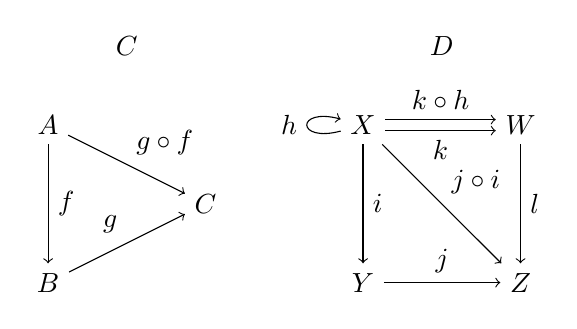
\begin{tikzpicture}[auto]
			\node (a) at (0, 2) {$A$};
			\node (b) at (0, 0) {$B$};
			\node (c) at (2, 1) {$C$};
			\draw[->] (a) to node{$f$}(b);
			\draw[->] (b) to node{$g$}(c);
			\draw[->] (a) to node{$g\circ f$}(c);

			\node (x) at (4, 2) {$X$};
			\node (y) at (4, 0) {$Y$};
			\node (w) at (6, 2) {$W$};
			\node (z) at (6, 0) {$Z$};
			\draw[->] (x) to node{$i$}(y);
			\draw[->] (y) to node{$j$}(z);
			\draw[->] (x) to node{$j\circ i$}(z);
			\draw[->] (w) to node{$l$}(z);
			\draw[->,transform canvas={yshift=-2pt}] (x) to node[swap]{$k$}(w);
			\draw[->,transform canvas={yshift=2pt}] (x) to node{$k\circ h$}(w);
			\draw[->,loop left ,looseness=10] (x) to node{$h$}(x);

			\node (catc) at (1, 3) {$\cat{C}$};
			\node (catd) at (5, 3) {$\cat{D}$};
		\end{tikzpicture}
	\end{center}
	関手$\functor{S,T}{C}{D}$を以下の対象と射の対応によって定義される関手とする。
	\begin{center}
		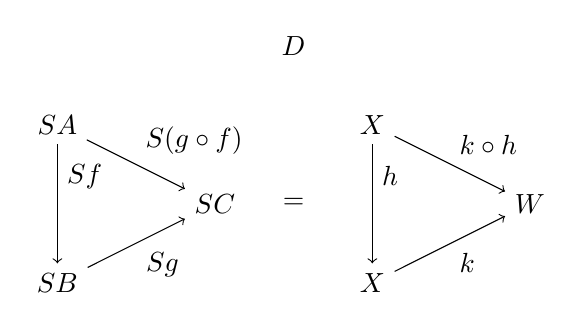
\begin{tikzpicture}[auto]
			\node (ta) at (4, 2) {$SA$};
			\node (tb) at (4, 0) {$SB$};
			\node (tc) at (6, 1) {$SC$};
			\node (x) at (8, 2) {$X$};
			\node (y) at (8, 0) {$X$};
			\node (z) at (10, 1) {$W$};

			\node (e) at (7, 1) {$=$};

			\draw[-, line width=4pt,draw=white] (x) to (y);
			\draw[->] (x) to node[yshift =10]{$h$}(y);
			\draw[->] (y) to node[swap]{$k$}(z);
			\draw[->] (x) to node{$k\circ h$}(z);

			\draw[-, line width=4pt,draw=white] (ta) to (tb);
			\draw[->] (ta) to node[yshift =10]{$Sf$}(tb);
			\draw[->] (tb) to node[swap]{$Sg$}(tc);
			\draw[->] (ta) to node{$S(g\circ f)$}(tc);

			\node (catd) at (7, 3) {$\cat{D}$};
		\end{tikzpicture}
	\end{center}
	\begin{center}
		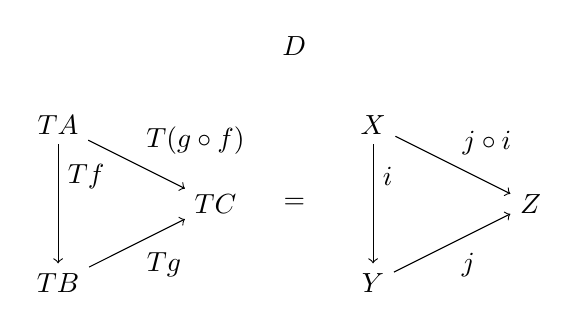
\begin{tikzpicture}[auto]
			\node (ta) at (4, 2) {$TA$};
			\node (tb) at (4, 0) {$TB$};
			\node (tc) at (6, 1) {$TC$};
			\node (x) at (8, 2) {$X$};
			\node (y) at (8, 0) {$Y$};
			\node (z) at (10, 1) {$Z$};

			\node (e) at (7, 1) {$=$};

			\draw[-, line width=4pt,draw=white] (x) to (y);
			\draw[->] (x) to node[yshift =10]{$i$}(y);
			\draw[->] (y) to node[swap]{$j$}(z);
			\draw[->] (x) to node{$j\circ i$}(z);

			\draw[-, line width=4pt,draw=white] (ta) to (tb);
			\draw[->] (ta) to node[yshift =10]{$Tf$}(tb);
			\draw[->] (tb) to node[swap]{$Tg$}(tc);
			\draw[->] (ta) to node{$T(g\circ f)$}(tc);

			\node (catd) at (7, 3) {$\cat{D}$};
		\end{tikzpicture}
	\end{center}
	関手$S,T$の間の自然変換$\natf{\alpha}{S}{T}{C}{D}$を以下の成分で定義する。
	\begin{align*}
		\mor{\alpha_A}{SA}{TA}&=\mor{h}{X}{X}\\
		\mor{\alpha_B}{SB}{TB}&=\mor{i}{X}{Y}\\
		\mor{\alpha_C}{SC}{TC}&=\mor{l}{W}{Z}
	\end{align*}
	\begin{center}
		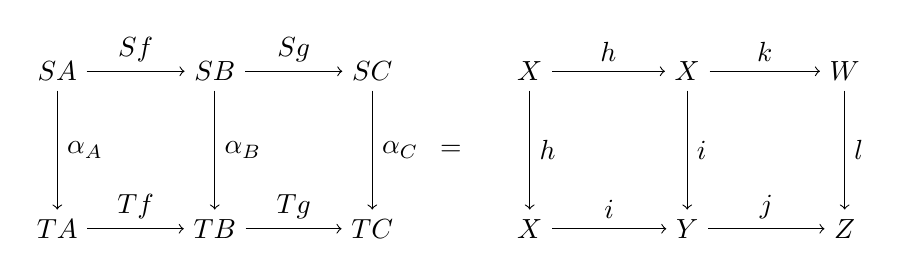
\begin{tikzpicture}[auto]
			\node (sa) at (0, 2) {$SA$};
			\node (sb) at (2, 2) {$SB$};
			\node (sc) at (4, 2) {$SC$};
			\node (ta) at (0, 0) {$TA$};
			\node (tb) at (2, 0) {$TB$};
			\node (tc) at (4, 0) {$TC$};
			\node (e) at (5, 1) {$=$};
			\draw[->] (sa) to node{$Sf$}(sb);
			\draw[->] (sb) to node{$Sg$}(sc);
			\draw[->] (ta) to node{$Tf$}(tb);
			\draw[->] (tb) to node{$Tg$}(tc);
			\draw[->] (sa) to node{$\alpha_A$}(ta);
			\draw[->] (sb) to node{$\alpha_B$}(tb);
			\draw[->] (sc) to node{$\alpha_C$}(tc);

			\node (sa') at (6, 2) {$X$};
			\node (sb') at (8, 2) {$X$};
			\node (sc') at (10, 2) {$W$};
			\node (ta') at (6, 0) {$X$};
			\node (tb') at (8, 0) {$Y$};
			\node (tc') at (10, 0) {$Z$};
			\draw[->] (sa') to node{$h$}(sb');
			\draw[->] (sb') to node{$k$}(sc');
			\draw[->] (ta') to node{$i$}(tb');
			\draw[->] (tb') to node{$j$}(tc');
			\draw[->] (sa') to node{$h$}(ta');
			\draw[->] (sb') to node{$i$}(tb');
			\draw[->] (sc') to node{$l$}(tc');
		\end{tikzpicture}
	\end{center}
	すると、
	\begin{align*}
		\alpha_B\circ Sf&=i\circ h\\
		&=Tf\circ\alpha_A\\
		\alpha_C\circ Sg&=l\circ k\\
		&=j\circ i\\
		&=Tg\circ\alpha_B
	\end{align*}
	となり、このような成分の定義は自然性を満たす。
	よって確かに$\alpha$は自然変換となる。

  \begin{define}[自然変換の同一性]
    二つの自然変換$\natf{\alpha,\beta}{F}{G}{C}{D}$が等しいとは、圏$\cat{C}$の任意の対象$X$に対して
    $\alpha_X=\beta_X$となるときである。
  \end{define}

  自然変換を対象による射の量化と捉えるならば、次に紹介する定関手の有用性がすぐに分かる。
  \begin{define}[定関手]
    圏$\cat{D}$の任意の対象$D$に対する\textbf{定関手}$\functor{\varDelta D}{C}{D}$を次のように定義する。
    \begin{quote}
			\begin{mydescription}
				\item[対象関数] 対象関数\[\mor{\varDelta D}{\obj{C}}{\obj{D}}\]
				を定写像$\mor{\varDelta D}{\obj{C}}{\obj{D}}$とする。すなわち圏$\cat{C}$の任意の対象$C$に対して$\varDelta D(C)=D$である。
				\item[射関数] 
        射関数は\[\mor{\varDelta D}{\arset{C}{A}{B}}{\arset{D}{\varDelta D(A)}{\varDelta D(B)}}\]であるが、対象関数の定義より、\[\mor{\varDelta D}{\arset{C}{A}{B}}{\arset{D}{D}{D}}\]と表せる。これを定写像$\mor{\varDelta id_A}{\arset{C}{A}{B}}{\arset{D}{D}{D}}$で定義する。\\
        すなわち、任意の射$\mor{f}{A}{B}$に対して$\varDelta D (f)=id_D$となる。
				\item[恒等射の保存] 射関数の定義より、任意の恒等射$id_C$に対して$\varDelta D (id_C)=id_D=id_{\varDelta D(C)}$であり成り立つ。
				\item[射の合成の保存] 同様に任意の合成可能な射$f,g$に対して、\[\varDelta D (g\circ f)=id_D=id_D\circ id_D=\varDelta D (g)\circ \varDelta D (f)\]であり成り立つ。
			\end{mydescription}
		\end{quote}
    \begin{center}
      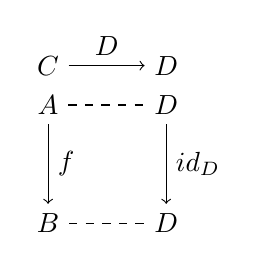
\begin{tikzpicture}[auto]
			  \node (catc) at (0, 2) {$\cat{C}$};
			  \node (catd) at (1.5, 2) {$\cat{D}$};
        \draw[->] (catc) to node{$\varDelta D$}(catd);
        \node (a) at (0, 1.5) {$A$};
        \node (b) at (0, 0) {$B$};
        \node (da) at (1.5, 1.5) {$D$};
        \node (db) at (1.5, 0) {$D$};
        \draw[->] (a) to node{$f$}(b);
        \draw[->] (da) to node{$id_D$}(db);
        \draw[-,dashed] (a) to (da);
        \draw[-,dashed] (b) to (db);
      \end{tikzpicture}
    \end{center}
  \end{define}
  次にある関手$\functor{F}{C}{D}$から$\functor{\varDelta D}{C}{D}$への自然変換$\nat{\alpha}{F}{\varDelta D}$を考えると、対象$A$に対する成分は$\mor{\alpha_A}{FA}{\varDelta D(A)}$であるから$\mor{\alpha_A}{FA}{D}$となり、射の始域のみを対象で量化することができることが分かる。また名前やその構成から分かるように、定関手は定写像の関手版である。
  \begin{center}
    \begin{tikzpicture}[auto]
      \node (A) at (0, 1) {$A$};
      \node (B) at (2, 1) {$B$};
      \node (FA') at (4, 2) {$FA$};
      \node (FB') at (6, 2) {$FB$};
      \node (GA') at (4, 0) {$\varDelta D(A)$};
      \node (GB') at (6, 0) {$\varDelta D(B)$};

      \node (FA) at (8, 2) {$FA$};
      \node (FB) at (10, 2) {$FB$};
      \node (GA) at (9, 0) {$D$};

			\node (e) at (7, 1) {$=$};
      \node (catc) at (1, 3) {$\cat{C}$};
      \node (catd) at (5, 3) {$\cat{D}$};

      \draw[->] (A) to node{$f$}(B);
      \draw[->] (FA) to node{$Ff$}(FB);
      \draw[->] (FA) to node[swap]{$\alpha_A$}(GA);
      \draw[->] (FB) to node{$\alpha_B$}(GA);
      \draw[->,loop below ,looseness=10] (GA) to node{$id_D$}(GA);

      \draw[->] (FA') to node{$Ff$}(FB');
      \draw[->] (GA') to node{$\varDelta D(f)$}(GB');
      \draw[->] (FA') to node[swap]{$\alpha_A$}(GA');
      \draw[->] (FB') to node{$\alpha_B$}(GB');
      \draw[->,bend left = 30] (catc) to node (funcf){$F$}(catd);
      \draw[->,bend right = 30] (catc) to node (funcg)[swap]{$\varDelta D$}(catd);
      \draw[double,double equal sign distance,-implies,shorten >=5pt,shorten <=5pt] (funcf) -- node[label=right:$\alpha$] {} (funcg);
    \end{tikzpicture}
  \end{center}

	ある圏$\cat{C}$の任意の対象$X$の恒等射$\mor{id_X}{X}{X}$はすべての対象に存在するため、対象$X$によって添字付けられた自然変換の成分$id$とみなせるかもしれない。
	実際に圏$\cat{C}$の二つの恒等関手$\functor{Id_C}{C}{C}$の間の自然変換\[\natf{id}{Id_C}{Id_C}{C}{C}\]を考えると、対象$X$に対する成分は$\mor{id}{Id(X)}{Id(X)}=\mor{id}{X}{X}$となる。
	また任意の射$\mor{f}{A}{B}$において\[id_B\circ f=f\circ id_A\]が成り立つから、確かに自然性を満たす。
	\begin{center}
		\begin{tikzpicture}[auto]
			\node (A) at (0, 1) {$A$};
			\node (B) at (2, 1) {$B$};
			\node (FA) at (4, 2) {$Id(A)$};
			\node (FB) at (6, 2) {$Id(B)$};
			\node (GA) at (4, 0) {$Id(A)$};
			\node (GB) at (6, 0) {$Id(B)$};

			\node (e) at (7.5, 1) {$=$};

			\node (catc) at (1, 4) {$\cat{C}$};
			\node (catd) at (5, 4) {$\cat{D}$};

			\draw[->] (A) to node{$f$}(B);
			\draw[->] (FA) to node{$Id(f)$}(FB);
			\draw[->] (GA) to node{$Id(f)$}(GB);
			\draw[->] (FA) to node{$id_A$}(GA);
			\draw[->] (FB) to node{$id_B$}(GB);

			\node (FA) at (8.5, 2) {$A$};
			\node (FB) at (10.5, 2) {$B$};
			\node (GA) at (8.5, 0) {$A$};
			\node (GB) at (10.5, 0) {$B$};
			\draw[->] (FA) to node{$id_A$}(GA);
			\draw[->] (FB) to node{$id_B$}(GB);
			\draw[->] (FA) to node{$f$}(FB);
			\draw[->] (GA) to node{$f$}(GB);
			\draw[->,bend left = 20] (catc) to node (funcf){$Id_C$}(catd);
			\draw[->,bend right = 20] (catc) to node (funcg)[swap]{$Id_C$}(catd);
			\draw[double,double equal sign distance,-implies,shorten >=5pt,shorten <=5pt] (funcf) -- node[label=right:$id$] {} (funcg);
		\end{tikzpicture}
	\end{center}
	次に自然変換$\natf{id}{Id_C}{Id_C}{C}{C}$を恒等関手$\functor{Id_C}{C}{C}$だけでなく、任意の関手$\functor{F}{C}{D}$で考えられるように一般化する。
	\begin{define}[恒等自然変換]
		関手$\functor{F}{C}{D}$に対して\textbf{恒等自然変換}$\natf{ID_F}{F}{F}{C}{D}$を、圏$C$の任意の対象$X$において\[(ID_F)_{X}=id_{FX}\]と定義する。

		これは\[(ID_F)_B\circ Ff=Ff\circ(ID_F)_A\]より自然性を満たす。
		\begin{center}
			\begin{tikzpicture}[auto]
				\node (A) at (0, 0.75) {$A$};
				\node (B) at (1.5, 0.75) {$B$};
				\node (FA) at (3, 1.5) {$FA$};
				\node (FB) at (4.5, 1.5) {$FB$};
				\node (GA) at (3, 0) {$FA$};
				\node (GB) at (4.5, 0) {$FB$};

				\node (catc) at (0.75, 3) {$\cat{C}$};
				\node (catd) at (3.75, 3) {$\cat{D}$};

				\draw[->] (A) to node{$f$}(B);
				\draw[->] (FA) to node{$Ff$}(FB);
				\draw[->] (GA) to node{$Ff$}(GB);
				\draw[->] (FA) to node[swap]{\scriptsize{$(ID_F)_A$}}(GA);
				\draw[->] (FB) to node{\scriptsize{$(ID_F)_B$}}(GB);

				\draw[->,bend left = 30] (catc) to node (funcf){$F$}(catd);
				\draw[->,bend right = 30] (catc) to node (funcg)[swap]{$F$}(catd);
				\draw[double,double equal sign distance,-implies,shorten >=5pt,shorten <=5pt] (funcf) -- node[label=right:$ID_F$] {} (funcg);
			\end{tikzpicture}
		\end{center}
	\end{define}

  自然変換は対象によって添字付けられた射の集合であったから、自然変換もまた一種の射のように振る舞う。次は自然変換の合成を、個々の成分の合成によって定義しようと思う。また後にこれがある圏における射の合成であることが分かるが、自然変換にはまた別の合成を考えることができるため、区別のため$\circ$ではなく$\cdot$と表記する。

	\begin{define}[自然変換の垂直合成]
		任意の関手$\functor{F,G,H}{C}{D}$の間の任意の自然変換$\nat{\alpha}{F}{G}$、$\nat{\beta}{G}{H}$の合成自然変換$\nat{\beta\cdot\alpha}{F}{H}$を、圏$\cat{C}$の任意の対象$X$における成分\[(\beta\cdot\alpha)_X=\mor{\beta_X\circ\alpha_X}{FX}{HX}\]によって定義する。
		\begin{center}
			\begin{tikzpicture}[auto]
				\node (A) at (0, 0) {$A$};
				\node (B) at (1.5, 0) {$B$};
				\node (FA) at (3, 1.5) {$FA$};
				\node (FB) at (4.5, 1.5) {$FB$};
				\node (GA) at (3, 0) {$GA$};
				\node (GB) at (4.5, 0) {$GB$};
				\node (HA) at (3, -1.5) {$HA$};
				\node (HB) at (4.5, -1.5) {$HB$};
				\node (catc) at (0.75, 3) {$\cat{C}$};
				\node (catd) at (3.75, 3) {$\cat{D}$};

				\draw[->] (A) to node{$f$}(B);
				\draw[->] (FA) to node{$Ff$}(FB);
				\draw[->] (GA) to node{$Gf$}(GB);
				\draw[->] (HA) to node{$Hf$}(HB);
				\draw[->] (FA) to node{$\alpha_A$}(GA);
				\draw[->] (FB) to node{$\alpha_B$}(GB);
				\draw[->] (GA) to node{$\beta_A$}(HA);
				\draw[->] (GB) to node{$\beta_B$}(HB);
				\draw[->,bend left = 50] (catc) to node (funcf){$F$}(catd);
				\draw[->] (catc) to node[yshift =-7,fill=white] (funcg){$G$}(catd);
				\draw[->,bend right = 50] (catc) to node (funch)[swap]{$H$}(catd);
				\draw[double,double equal sign distance,-implies,shorten >=2pt,shorten <=3pt] (funcf) -- node[label=right:$\alpha$] {} (funcg);
				\draw[double,double equal sign distance,-implies,shorten >=3pt,shorten <=2pt] (funcg) -- node[label=right:$\beta$] {} (funch);
			\end{tikzpicture}
			\begin{tikzpicture}[auto]
				\node (A) at (0, 0) {$A$};
				\node (B) at (1.5, 0) {$B$};
				\node (FA) at (3, 1.5) {$FA$};
				\node (FB) at (4.5, 1.5) {$FB$};
				\node (HA) at (3, -1.5) {$HA$};
				\node (HB) at (4.5, -1.5) {$HB$};
				\node (catc) at (0.75, 3) {$\cat{C}$};
				\node (catd) at (3.75, 3) {$\cat{D}$};

				\draw[->] (A) to node{$f$}(B);
				\draw[->] (FA) to node{$Ff$}(FB);
				\draw[->] (HA) to node{$Hf$}(HB);
				\draw[->] (FA) to node{$\beta_A\circ\alpha_A$}(HA);
				\draw[->] (FB) to node{$\beta_B\circ\alpha_B$}(HB);
				\draw[->,bend left = 50] (catc) to node (funcf){$F$}(catd);
				\draw[->,bend right = 50] (catc) to node (funch)[swap]{$H$}(catd);
				\draw[double,double equal sign distance,-implies,shorten >=5pt,shorten <=5pt] (funcf) -- node[label=right:$\alpha\cdot\beta$] {} (funch);
			\end{tikzpicture}
		\end{center}
		すると任意の射$\mor{f}{A}{B}$において
		\begin{align*}
			(\beta\cdot\alpha)_B\circ Ff&=\beta_B\circ\alpha_B\circ Ff&\text{(合成自然変換の成分)}\\
			&=\beta_B\circ Gf\circ \alpha_A&\text{($\alpha$の自然性)}\\
			&=Hf\circ\beta_A\circ\alpha_A&\text{($\beta$の自然性)}\\
			&=Hf\circ(\beta\cdot\alpha)_A&\text{(合成自然変換の成分)}
		\end{align*}
		となり、$\beta\cdot\alpha$は確かに自然性を満たす。
	\end{define}

  自然変換によって量化された対象や射の性質を同時に述べることができると書いたが、実際に積関手と射影関手の間の自然変換を考えることによって、個々の積対象の持つ射影射の性質の一部を述べようと思う。

	\begin{prop}[射影射の自然性]
		積を持つ圏$\cat{C}$の任意の積$A\times B$の射影射$\mor{\pi_{L,\tuple{A,B}}}{A\times B}{A}$は、双積関手$\functor{(-\times -)}{C\times C}{C}$から射影関手$\functor{\Pi_{L,\tuple{\cat{C,C}}}}{C\times C}{C}$への自然変換の成分である。

		この自然変換を\[\nat{\pi_L}{(-\times -)}{\Pi_{L\tuple{\cat{C,C}}}}\]とし、成分を\[(\pi_L)_{A\times B}=\mor{\pi_{LA}}{A\times B}{A}\]とする。
		すると、射の積の定義$f\times g = \tuple{f\circ\pi_{LA},g\circ\pi_{RB}}$より、
		\begin{align*}
			(\pi_L)_{A'\times B'}\circ (f\times g)&=\pi_{LA}\circ (f\times g)&\text{(成分の定義)}\\
			&=\pi_{LA}\circ\tuple{f\circ\pi_{LA},g\circ\pi_{RB}}&\text{(射の積の定義)}\\
			&=f\circ\pi_{LA}&\text{(射の対の可換性)}\\
			&=f\circ(\pi_L)_{A\times B}&\text{(成分の定義)}
		\end{align*}
		となり、確かに自然性を満たす。
		\begin{center}
			\begin{tikzpicture}[auto]
				\node (ab) at (0, 1) {$\pcobj{A,B}$};
				\node (a'b') at (2, 1) {$\pcobj{A',B'}$};
				\draw[->] (ab) to node{$\pcobj{f,g}$}(a'b');

				\node (pab) at (4, 2) {$A\times B$};
				\node (pa'b') at (6, 2) {$A'\times B'$};
				\node (a) at (4, 0) {$A$};
				\node (a') at (6, 0) {$A'$};
				\draw[->] (pab) to node{$f\times g$}(pa'b');
				\draw[->] (a) to node{$f$}(a');
				\draw[->] (pab) to node{$(\pi_L)_{A\times B}$}(a);
				\draw[->] (pa'b') to node{$(\pi_L)_{A'\times B'}$}(a');

				\node (catcc) at (1, 3.5) {$\cat{C\times C}$};
				\node (catc) at (5, 3.5) {$\cat{C}$};

				\draw[->,bend left = 20] (catcc) to node (funcf){$(-\times -)$}(catc);
				\draw[->,bend right = 20] (catcc) to node (funch)[swap]{$\Pi_{LC}$}(catc);
				\draw[double,double equal sign distance,-implies,shorten >=5pt,shorten <=5pt] (funcf) -- node[label=right:$\pi_L$] {} (funch);
			\end{tikzpicture}
		\end{center}
	\end{prop}

  関手の射集合を厳密に表記すると$\mor{F_{A,B}}{\arset{C}{A}{B}}{\arset{D}{FA}{FB}}$のように添字がつくが、これも少し複雑ではあるが実際に自然変換になる。

	\begin{prop}[関手の射関数の自然性]
		ある関手$\functor{F}{C}{D}$圏$\cat{C}$の任意の二対象$A,B$に対して\[\mor{F_{A,B}}{\arset{C}{A}{B}}{\arset{D}{FA}{FB}}\]となる射関数は\[\natf{F}{\arset{C}{-}{-}}{\arset{D}{F-}{F-}}{C^{op}\times C}{Set}\]となるような自然変換である。
		
		また関手$\arset{D}{F-}{F-}$は\[\arset{D}{F-}{F-}=\arset{D}{-}{-}\circ (F^{op}\times F)\]と定義される。具体的な対応は下の図式で確認してほしい。
		
		\begin{center}
			\begin{tikzpicture}[auto]
				\node (ab) at (0, 1) {$\pcobj{A,B}$};
				\node (a'b') at (2, 1) {$\pcobj{A',B'}$};
				
				\node (cab) at (4, 2) {$\arset{C}{A}{B}$};
				\node (ca'b') at (7, 2) {$\arset{C}{A'}{B'}$};
				
				\node (dab) at (4, 0) {$\arset{D}{FA}{FB}$};
				\node (da'b') at (7, 0) {$\arset{D}{FA'}{FB'}$};				
				\draw[->] (ab) to node{$\pcobj{f,g}$}(a'b');
				\draw[->] (cab) to node{$\arset{C}{f}{g}$}(ca'b');
				\draw[->] (dab) to node{$\arset{D}{Ff}{Fg}$}(da'b');
				
				\draw[->] (cab) to node{$F_{A,B}$}(dab);				\draw[->] (ca'b') to node{$F_{A',B'}$}(da'b');				\node (catcc) at (1, 3.5) {$\cat{C\times C^{op}}$};
				\node (catc) at (5.5, 3.5) {$\cat{Set}$};
				
				\draw[->,bend left = 20] (catcc) to node (funcf){$\arset{C}{-}{-}$}(catc);
				\draw[->,bend right = 20] (catcc) to node (funch)[swap]{$\arset{D}{F-}{F-}$}(catc);
				\draw[double,double equal sign distance,-implies,shorten >=5pt,shorten <=5pt] (funcf) -- node[label=right:$F$] {} (funch);
			\end{tikzpicture}
		\end{center}
	\end{prop}
	\begin{proof}
		射関数の定義より、$F_{A,B}$のような射は任意の対象に対して存在する。そのため自然変換$F$の成分とみなすことができる。
		自然性は上の図式が可換、つまり\[F_{A',B'}\circ\arset{C}{f}{g}=\arset{D}{Ff}{Fg}\circ F_{A,B}\]を示せば良い。この図式は$\cat{Set}$上にあるため、元の対応関係から射の等式を導く。
		圏$\cat{C}$の任意の射$\mor{f}{A}{B}$に対して
		\begin{align*}
			F_{A',B'}\circ\arset{C}{f}{g}(h)&=F_{A',B'}(g\circ h\circ f)&\text{(射写像の定義)}\\
			&=Fg\circ Fh\circ Ff&\text{(関手の射の合成の保存)}\\
			&=\arset{D}{Ff}{Fg}(Fh)&\text{(射写像の定義)}\\
			&=\arset{D}{Ff}{Fg}\circ F_{A,B}(h)&\text{(表記揺れ)}
		\end{align*}
		$F_{A',B'}\circ\arset{C}{f}{g}(h)=\arset{D}{Ff}{Fg}\circ F_{A,B}(h)$より自然性が成り立つから、確かに射関数の全体は自然変換となる。
	\end{proof}
	この証明では関手$F$は関手$\arset{D}{F-}{F-}$の定義と自然変換と見なした射関数の二つに現れている。そのため、関手$F$が純粋に自然変換から構成できる主張することはできないが、関手$\arset{C}{-}{-}$と関手$\arset{D}{F-}{F-}$の間の射関数となるような自然変換はただ一つである。これは射関数$F_{A,A}$の恒等射の保存から示すことができるので、余力があれば証明してみてほしい。

  \begin{prop}[評価射の自然性]
    評価射$\mor{ev_{A,B}}{\arset{Set}{B}{A}\times B}{A}$は$A$に対して自然である。
  \end{prop}
  \begin{proof}
    成分$ev_{A,B}$によって構成される自然変換を$\nat{ev_B}{\arset{Set}{B}{-}\times B}{Id_{\cat{Set}}}$とする。\\
    また、$\arset{Set}{B}{-}\times B$は積関手$(-)\times B$と、Hom関手$\arset{Set}{B}{-}$の合成関手$((-)\times B)\circ\arset{Set}{B}{-}$とする。すなわち、
    \begin{align*}
      \arset{Set}{B}{-}\times B(A)&=((-)\times B)\circ\arset{Set}{B}{-}(A)\\
      &=((-)\times B)(\arset{Set}{B}{A})\\
      &=\arset{Set}{B}{A}\times B\\
    \end{align*}となる。\\
    このような評価射が任意の対象に対して存在することは明らかであるから、あとは自然性を証明すればよい。\\
    任意の射$\mor{g}{A}{A'}$に対して$g\circ ev_{A,B} = ev_{A',B}\circ (\arset{Set}{B}{g}\times id_B)$を示す。任意の射$\mor{f}{B}{A}$と$B$の任意の元$b$の対$\tuple{f,b}$に対して、
    \begin{align*}
      g\circ ev_{A,B}(\tuple{f,b})&=g(f(b))&\text{(評価射の定義)}\\
      &=(g\circ f)(b)&\text{(写像の合成の定義)}\\
      &=ev_{A',B}(\tuple{g\circ f, b})&\text{(評価射の定義)}\\
      &=ev_{A',B}((\arset{Set}{B}{g}\times id_B)(\tuple{f,b}))&\text{(射の積の定義)}\\
      &=ev_{A',B}\circ (\arset{Set}{B}{g}\times id_B)(\tuple{f,b})\\
    \end{align*}
    このように写像の合成の定義の等式によって自然性を満たす。よって評価射が自然変換の成分であることが分かった。
    \begin{center}
			\begin{tikzpicture}[auto]
				\node (ab) at (0, 1) {$A$};
				\node (a'b') at (2, 1) {$A'$};
				
				\node (cab) at (4, 2) {$\arset{Set}{B}{A}\times B$};
				\node (ca'b') at (7, 2) {$\arset{Set}{B}{A'}\times B$};
				
				\node (dab) at (4, 0) {$A$};
				\node (da'b') at (7, 0) {$A'$};				
				\draw[->] (ab) to node{$g$}(a'b');
				\draw[->] (cab) to node[yshift = 4]{$\arset{Set}{B}{g}\times id_B$}(ca'b');
				\draw[->] (dab) to node{$g$}(da'b');
				\draw[->] (cab) to node{$ev_{A,B}$}(dab);
        \draw[->] (ca'b') to node{$ev_{A',B}$}(da'b');				\node (catcc) at (1, 3.5) {$\cat{Set}$};
				\node (catc) at (5.5, 3.5) {$\cat{Set}$};
				
				\draw[->,bend left = 20] (catcc) to node (funcf){$\arset{Set}{B}{-}\times B$}(catc);
				\draw[->,bend right = 20] (catcc) to node (funch)[swap]{$Id_\cat{Set}$}(catc);
				\draw[double,double equal sign distance,-implies,shorten >=5pt,shorten <=5pt] (funcf) -- node[label=right:$ev_B$] {} (funch);
			\end{tikzpicture}
		\end{center}

  \end{proof}
  \begin{prop}[余評価射の自然性]
    余評価射$\mor{ce_{A,B}}{A}{\arset{Set}{B}{A\times B}}$は$A$に対して自然である。
  \end{prop}
  \begin{proof}
    評価射と同様に示す。\\
    $\arset{Set}{B}{-\times B} = \arset{Set}{B}{-}\circ (-\times B)$とすると、$\arset{Set}{B}{-\times B}(A)=\arset{Set}{B}{A\times B}$である。これにより成分$ce_{A,B}$によって構成される自然変換を$\mor{ce_B}{Id_{\cat{Set}}}{\arset{Set}{B}{-\times B}}$とする。同様に任意の射$\mor{f}{A}{A'}$に対して$\arset{Set}{B}{f\times id_B}\circ ce_{A,B}=ce_{A',B}\circ f$が成り立つことを示す。対象$A$の任意の元を$a$とすると、
    \begin{align*}
      \arset{Set}{B}{f\times id_B}\circ ce_{A,B}(a)&=\arset{Set}{B}{f\times id_B}(\lambda x.\tuple{a,x})&\text{(余評価射の定義)}\\
      &=(f\times id_B)\circ(\lambda x.\tuple{a,x})&\text{(Hom関手の定義)}\\
      &=\lambda x.(f\times id_B)(\tuple{a,x})&\text{(表記変更)}\\
      &=\lambda x.\tuple{f(a),x}&\text{(射の積の定義)}\\      
      (ce_{A',B}\circ f)(a)&=ce_{A',B}(f(a))&\text{(写像の合成の定義)}\\
      &=\lambda x.\tuple{f(a),x}&\text{(余評価射の定義)}
    \end{align*}
    $\arset{Set}{B}{f\times id_B}\circ ce_{A,B}(a)=\lambda x.\tuple{f(a),x}$と$(ce_{A',B}\circ f)(a)=\lambda x.\tuple{f(a),x}$が示せたわけだが、$\lambda x.\tuple{f(a),x}$は表記が一致しただけあって直ちに$\arset{Set}{B}{f\times id_B}\circ ce_{A,B}=ce_{A',B}\circ f$が示せるわけでは無いが、定義を考えると明らかに等しい。よって余評価射は自然変換の成分である。
    \begin{center}
			\begin{tikzpicture}[auto]
				\node (ab) at (0, 1) {$A$};
				\node (a'b') at (2, 1) {$A'$};
				
				\node (cab) at (4, 2) {$A$};
				\node (ca'b') at (7, 2) {$A'$};
				
				\node (dab) at (4, 0) {$\arset{Set}{B}{A\times B}$};
				\node (da'b') at (7, 0) {$\arset{Set}{B}{A'\times B}$};				
				\draw[->] (ab) to node{$f$}(a'b');

				\draw[->] (cab) to node{$f$}(ca'b');
				\draw[->] (dab) to node[swap, yshift = -4]{$\arset{Set}{B}{f\times id_B}$}(da'b');

				\draw[->] (cab) to node{$ev_{A,B}$}(dab);
        \draw[->] (ca'b') to node{$ev_{A',B}$}(da'b');				\node (catcc) at (1, 3.5) {$\cat{Set}$};
				\node (catc) at (5.5, 3.5) {$\cat{Set}$};
				
				\draw[->,bend left = 20] (catcc) to node (funcf){$Id_{\cat{Set}}$}(catc);
				\draw[->,bend right = 20] (catcc) to node (funch)[swap]{$\arset{Set}{B}{-\times B}$}(catc);
				\draw[double,double equal sign distance,-implies,shorten >=5pt,shorten <=5pt] (funcf) -- node[label=right:$ev_B$] {} (funch);
			\end{tikzpicture}
		\end{center}
  \end{proof}
  $ev_{A,B}$と$ce_{A,B}$がAに対して自然であることを述べたが、このような射は任意の$B$に対しても定義できる。しかし$B$は関手の始域、終域の片方のみに二つの同じ対象が現れている。同じ対象というのは例えば評価射の場合、$\mor{ev_{A,B}}{\arset{Set}{B}{A}\times B'}{A}$となるような評価射は構成できない。このような制約を関手で行うこともできるが、一般的にはこのような自然性も許容した超自然変換と呼ばれる自然変換の一般化によって定義され、自然変換と同様の性質を持つ。
	\subsection{関手圏}
	自然変換には恒等射によって定義される恒等自然変換と、射の合成によって定義される垂直変換を考えることができた。これまで様々な圏を考えてきたように、これらの自然変換を用いれば実際に圏を考えることができるようになる。
	\begin{define}[関手圏]
		二つの圏$\cat{C,D}$に対する\textbf{関手圏}$\funccat{C}{D}$を以下の要素で定義する。
		\begin{quote}
			\begin{mydescription}
				\item[対象] $\obj{\funccat{C}{D}}$を$\cat{C}$から$\cat{D}$への関手の全体とする。すなわち、$\cat{Cat}$における射集合によって$\obj{\funccat{C}{D}}=\arset{Cat}{\cat{C}}{\cat{D}}$と表せる。
				\item[射]任意の関手$\functor{F,G}{C}{D}$に対して、射集合$\arset{\funccat{C}{D}}{F}{G}$を関手$F,G$の間の自然変換全体の集合とする。
				\item[射の合成] 任意の関手$\functor{F,G,H}{C}{D}$の間の任意の自然変換$\nat{\alpha}{F}{G}$、$\nat{\beta}{G}{H}$を合成した自然変換を、自然変換の垂直合成によって$\beta\cdot\alpha$と定義する。
				\item[恒等射の存在]任意の関手$\functor{F}{C}{D}$に対して、恒等射となる自然変換を恒等自然変換によって$ID_F$と定義する。
				\item[結合律]任意の関手$\functor{F,G,H,I}{C}{D}$と自然変換$\nat{\alpha}{F}{G}$、$\nat{\beta}{G}{H}$、$\nat{\gamma}{H}{I}$に対して、\[(\gamma\cdot\beta)\cdot\alpha=\gamma\cdot(\beta\cdot\alpha)\]が成り立てば良い。
				自然変換の成分はただの射であるから圏$\cat{D}$の結合律より、圏$\cat{C}$の任意の対象$X$に対して

        \begin{align*}
          ((\gamma\cdot\beta)\cdot\alpha)_X&=(\gamma_X\circ\beta_X)\circ\alpha_X&\text{(自然変換の垂直合成の定義)}\\
          &=\gamma_X\circ(\beta_X\circ\alpha_X)&\text{(圏$\cat{D}$の結合律)}\\
          &=(\gamma\cdot(\beta\cdot\alpha))_X&\text{(自然変換の垂直合成の定義)}\\
        \end{align*}
        が成り立つ。よって二つの自然変換のすべての成分が一致するから$(\gamma\cdot\beta)\cdot\alpha=\gamma\cdot(\beta\cdot\alpha)$であり、結合律が成り立つ。
				\item[単位元律] 任意の関手$\functor{G}{C}{D}$に対応する恒等自然変換$ID_G$と、任意の関手$\functor{F,H}{C}{D}$、任意の自然変換$\nat{\alpha}{F}{G}$、$\nat{\beta}{G}{H}$に対して、
        \[ID_G\cdot\alpha=\alpha,\, \beta\cdot ID_G=\beta\]が成り立つことを示せば良い。
				結合律と同様に成分を考える。恒等自然変換の成分は恒等射であるから、圏$\cat{C}$の任意の対象$X$に対して
        \begin{align*}
          (ID_G\cdot\alpha)_X&=(ID_G)_X\circ\alpha_X&\text{(自然変換の垂直合成の定義)}\\
          &=id_{GX}\circ\alpha_X&\text{恒等自然変換の定義}\\
          &=\alpha_X&\text{圏$\cat{D}$の単位元律}
        \end{align*}
        $\beta$に対しても同様に示せる。よって$ID_G\cdot\alpha=\alpha,\, \beta\cdot ID_G=\beta$であり、単位元律が成り立つ。
			\end{mydescription}
		\end{quote}
	\end{define}
  まだ圏論的な操作からは関手圏を定義することはできないが、関手圏の対象の集合や射集合が定義できることは関手、自然変換が写像、射集合を用いて定義されていることから簡単に分かる。

  関手圏が圏であるということは、関手圏は$\cat{Cat}$の対象である。つまりある圏からある関手圏への関手を考えることができるようになる。その一例として定写像から対角写像を得たように、定関手を得る操作を関手と見なした対角関手を見ていこう。\\
  \begin{define}[対角関手]
    圏$\cat{C}$から$\cat{D}$への定関手を与える対角関手$\functor{\varDelta}{D}{\funccat{C}{D}}$を以下のように定義する。
    \begin{quote}
			\begin{mydescription}
				\item[対象関数] 対象関数\[\mor{\varDelta}{\obj{D}}{\obj{\funccat{C}{D}}}\]
				を圏$\cat{D}$の任意の対象$D$と定関手$\functor{\varDelta D}{C}{D}$に対して定関数$\varDelta(D)=\varDelta D$と定義する。またここでの$\varDelta D$は射関数ではなく
				\item[射関数] 
        射関数は\[\mor{\varDelta}{\arset{C}{A}{B}}{\arset{\funccat{C}{D}}{\varDelta A}{\varDelta B}}\]となるように、$A$から$B$への射を、$A$の定関手から$B$の定関手への自然変換に写す写像になる。またこの自然変換を射$f$に対する定自然変換と呼ぶことにする。

        まずは任意の射$\mor{f}{A}{B}$に対する定自然変換$\nat{\varDelta f}{\varDelta A}{\varDelta B}$を先に定義する。
        圏$\cat{C}$の任意の対象$C$に対する$\varDelta f$の成分は\[\mor{(\varDelta f)_C}{\varDelta A(C)}{\varDelta B(C)}\]となるが、定関手の定義より、\[\mor{(\varDelta f)_C}{A}{B}\]と表せる。つまり、二つの定関手によって定自然変換の始域と終域がそれぞれ$A,B$に集約されているため成分を$(\varDelta f)_C=f$と定義できる。

        自然性については、\[(\varDelta f)_{C'}\circ\varDelta A(g)=f\circ id_A=id_B\circ f=\varDelta B(g)\circ(\varDelta f)_C\]と成り立ち、$\varDelta f$が自然変換であることが分かった。

        \begin{center}
          \begin{tikzpicture}[auto]
            \node (A) at (0, 1) {$C$};
            \node (B) at (2, 1) {$C'$};
            \node (FA') at (4, 2) {$\varDelta A(C)$};
            \node (FB') at (6, 2) {$\varDelta A(C')$};
            \node (GA') at (4, 0) {$\varDelta B(C)$};
            \node (GB') at (6, 0) {$\varDelta B(C')$};
      
            \node (FA) at (8, 2) {$A$};
            \node (FB) at (10, 2) {$A$};
            \node (GA) at (8, 0) {$B$};
            \node (GB) at (10, 0) {$B$};

            \node (e) at (7, 1) {$=$};
            \node (catc) at (1, 3.5) {$\cat{C}$};
            \node (catd) at (5, 3.5) {$\cat{D}$};
      
            \draw[->] (A) to node{$g$}(B);

            \draw[->] (FA) to node{$id_A$}(FB);
            \draw[->] (FA) to node[swap]{$f$}(GA);
            \draw[->] (FB) to node{$f$}(GB);
            \draw[->] (GA) to node{$id_B$}(GB);

            \draw[->] (FA') to node{$\varDelta A(g)$}(FB');
            \draw[->] (GA') to node{$\varDelta B(g)$}(GB');
            \draw[->] (FA') to node[swap]{$(\varDelta f)_C$}(GA');
            \draw[->] (FB') to node[swap]{$(\varDelta f)_C'$}(GB');
            \draw[->,bend left = 20] (catc) to node (funcf){$\varDelta A$}(catd);
            \draw[->,bend right = 20] (catc) to node (funcg)[swap]{$\varDelta B$}(catd);
            \draw[double,double equal sign distance,-implies,shorten >=5pt,shorten <=5pt] (funcf) -- node[label=right:$\varDelta f$] {} (funcg);
          \end{tikzpicture}
        \end{center}

        これによって、対角関手の射関数$\mor{\varDelta}{\arset{C}{A}{B}}{\arset{\funccat{C}{D}}{\varDelta A}{\varDelta B}}$を$\varDelta(f)=\varDelta f$と定義する。

				\item[恒等射の保存] 圏$\cat{D}$の任意の対象$D$に対して$\varDelta(id_D)=ID_{\varDelta D}$を示せば良い。また対角関手の終域は関手圏であるため、関手圏の恒等射である恒等自然変換に対応する。
        圏$\cat{C}$の任意の対象$C$の成分を見ると、
        \begin{align*}
          (\varDelta (id_D))_C &= id_D &\text{(射関数の定義)}\\
          (ID_{\varDelta D})_C &= id_{\varDelta D(C)}&\text{(恒等自然変換の定義)}\\
          &= id_D&\text{(定関手の定義)}
        \end{align*}
        よって任意の成分について\[(\varDelta (id_D))_C=id_D=(ID_{\varDelta D})_C\]が成り立つから$\varDelta(id_D)=ID_{\varDelta D}$となり、恒等射を保存する。

				\item[射の合成の保存] 圏$\cat{D}$の合成可能な二射$f,g$に対して、$\varDelta(g\circ f)=\varDelta g\circ \varDelta f$が成り立てばよい。同様に圏$\cat{C}$の任意の対象$C$に対する成分を見ると、
        \begin{align*}
          (\varDelta(g\circ f))_C&=g\circ f&\text{(射関数の定義)}\\
          (\varDelta g\cdot\varDelta f)_C &= (\varDelta g)_C\circ (\varDelta f)_C&\text{(自然変換の垂直合成の定義)}\\
          &=g\circ f&\text{(射関数の定義)}
        \end{align*}
        よって任意の成分について\[(\varDelta(g\circ f))_C=g\circ f=(\varDelta g)_C\circ (\varDelta f)_C\]が成り立つから$\varDelta(g\circ f)=\varDelta g\circ \varDelta f$となり、射の合成を保存する。
			\end{mydescription}
		\end{quote}
  \end{define}

  圏から関手圏への関手が違和感なく定義される事が分かったと思う。次は更に踏み込んで圏と関手圏の間の同型を示す。\\
  また圏の同型についても軽く触れておこう。
  \begin{define}[圏同型]
    $\cat{Cat}$において、圏$\cat{C,D}$が関手$\functor{I}{C}{D},\ \functor{I^{-1}}{D}{C}$によって同型、つまり$I\circ I^{-1}=Id_D,\ I^{-1}\circ I=Id_C$である時、圏同型と呼ぶことにする。またこの時関手$I,I^{-1}$を\textbf{同型関手}と呼ぶことにする。
  \end{define}
  一般の圏と同様に元の対応を見てみよう。同型の元の関係より、$\functor{C}{1}{C}$は$\cat{C}$の対象と同一視できるのだった。すなわちある対象$D$が存在して$C\sim D$となる。\\

  \begin{center}
    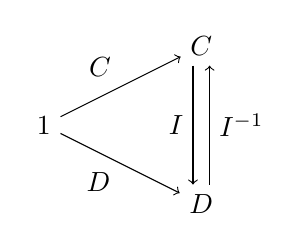
\begin{tikzpicture}[auto]
      \node (1) at (-2, 1) {$\cat{1}$};
      \node (a) at (0, 2) {$\cat{C}$};
      \node (b) at (0, 0) {$\cat{D}$};
      \draw[->] (1) to node{$C$}(a);
      \draw[->] (1) to node[swap]{$D$}(b);
      \draw[->,transform canvas={xshift=-3pt}] (a) to node[swap] {$I$}(b);
      \draw[->,transform canvas={xshift=3pt}] (b) to node[swap] {$I^{-1}$}(a);
    \end{tikzpicture}
  \end{center}
  関手の定義に乗っ取ると、関手$I\circ I^{-1}$の対象関数は合成関手の定義より、それぞれの対象関数\[\mor{I}{\obj{C}}{\obj{D}},\ \mor{I^{-1}}{\obj{D}}{\obj{C}}\]の合成\[\mor{I\circ I^{-1}}{\obj{D}}{\obj{D}}\]が対象関数になる。$I\circ I^{-1}=Id_\cat{D}$であるから、対象関数においても$I\circ I^{-1}=id_{\obj{D}}$が成り立つ。同様に$I^{-1}\circ I=id_{\obj{C}}$も成り立つから、$I,I^{-1}$の対象関数も$\cat{Set}$上の同型射となる。

  次に圏の射の対応関係を見ていこう。
  関手の定義に従って考えると、関手$I\circ I^{-1}$の射関数は、合成関手の定義よりそれぞれの射関数$\mor{I}{\arset{C}{A}{B}}{\arset{D}{IA}{IB}}$、$\mor{I^{-1}}{\arset{D}{A}{B}}{\arset{C}{I^{-1}A}{I^{-1}B}}$の合成射
  \[\mor{I\circ I^{-1}}{\arset{D}{A}{B}}{\arset{D}{A}{B}}\]が射関数となる。対象関数と同様にこれも同型射になるから、射$\mor{f}{C}{C'}$に対して$Ff=g,\ C\sim D, C'\sim D'$とすると同型$\arset{C}{C}{C'}\cong\arset{D}{D}{D'}$によって$f\sim g$と表記できる。
  \begin{center}
    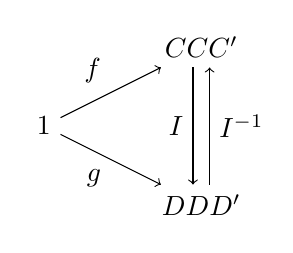
\begin{tikzpicture}[auto]
      \node (1) at (-2, 1) {$1$};
      \node (a) at (0, 2) {$\arset{C}{C}{C'}$};
      \node (b) at (0, 0) {$\arset{D}{D}{D'}$};
      \draw[->] (1) to node{$f$}(a);
      \draw[->] (1) to node[swap]{$g$}(b);
      \draw[->,transform canvas={xshift=-3pt}] (a) to node[swap] {$I$}(b);
      \draw[->,transform canvas={xshift=3pt}] (b) to node[swap] {$I^{-1}$}(a);
    \end{tikzpicture}
  \end{center}  
  \begin{prop}[圏の元]
    一点離散圏$\cat{1}$、任意の圏$\cat{C}$に対して$\cat{C}\cong\funccat{1}{C}$
  \end{prop}
  \begin{proof}
    集合の圏における同型$A\cong\arset{Set}{1}{A}$と同様の手法で証明する。
    すなわち、対角関手$\functor{\varDelta}{C}{\funccat{1}{C}}$が同型射となる関手であることを示す。\\
    また定写像と同様に$\funccat{1}{C}$の対象である任意の関手は明らかに定関手である。なぜなら一点離散圏$\cat{1}$はただ一つの対象と射のみを持ち、それらは必ず圏$\cat{C}$のただ一つの対象とその恒等射に写されるため、定関手の定義を満たす。\\
    関手$\functor{\varDelta^{-1}}{C^1}{C}$を
    \begin{quote}
			\begin{mydescription}
				\item[対象関数]対象関数\[\mor{\varDelta^{-1}}{\obj{C^1}}{\obj{C}}\]を圏$\funccat{C}{1}$の任意の対象$\varDelta A$に対して$\varDelta^{-1}(\varDelta A)=\varDelta A(*)=A$と定義する。\\
        この対象関数の全域性は先ほど示した$\funccat{C}{1}$の性質によるものである。
				\item[射関数]射関数\[\mor{\varDelta^{-1}}{\arset{\funccat{1}{C}}{\varDelta A}{\varDelta B}}{\arset{C}{A}{B}}\]を任意の定自然変換$\nat{\varDelta f}{\varDelta A}{\varDelta B}$に対して$\varDelta^{-1}(\varDelta f) = (\varDelta f)_*=f$と定義する。
				\item[恒等射の保存]任意の対象$A$に対して$\varDelta^{-1}(ID_{\varDelta_A})=id_{\varDelta^{-1}(\varDelta A)}$を示せばよい。これは対角関手の恒等射の保存から簡単に示せる。
				\begin{align*}
          \varDelta^{-1}(ID_{\varDelta A})&=\varDelta^{-1}(\varDelta id_A)&\text{(対角関手の恒等射の保存)}\\
          &=id_A&\text{(射関数の定義)}\\
          &=id_{\varDelta^{-1}(\varDelta A)}&\text{(対象関数の定義)}
        \end{align*}
        よって成り立つ。
				\item[射の合成の保存]任意の合成可能な二射$f,g$に対して、$\varDelta^{-1}(\varDelta g\cdot\varDelta f)=\varDelta^{-1}(\varDelta g)\circ\varDelta^{-1}(\varDelta f)$が成り立つことを示せばよい。同様に対角関手の射の合成の保存から簡単に示せる。
				\begin{align*}
          \varDelta^{-1}(\varDelta g\cdot\varDelta f)&=\varDelta^{-1}(\varDelta(g\circ f))&\text{(対角関手の射の合成の保存)}\\
          &=g\circ f&\text{(射関数の定義)}\\
          &=\varDelta^{-1}(\varDelta g)\circ\varDelta^{-1}(\varDelta f)&\text{(射関数の定義)}
        \end{align*}
			\end{mydescription}
		\end{quote}
    対象関数$\varDelta,\ \varDelta^{-1}$において、圏$\cat{C}$の任意の対象$A$に対して
    \begin{align*}
      A&=\varDelta^{-1}(\varDelta A)\\
      &=(\varDelta^{-1}\circ\varDelta)(A)
    \end{align*}
    であるから、$\varDelta^{-1}\circ\varDelta=id_\obj{C}$が成り立つ。\\
    圏$\funccat{C}{1}$の任意の対象$F$を考えるが、$\funccat{C}{1}$の任意の対象は定関手であるため、任意の定関手$\varDelta A$を考えればよい。よって
    \begin{align*}
      F&=\varDelta A\\
      &=\varDelta((\varDelta^{-1}\circ\varDelta)(A))\\
      &=(\varDelta\circ \varDelta^{-1})(\varDelta A)\\
      &=(\varDelta\circ \varDelta^{-1})(F)
    \end{align*}
    よって、$\varDelta\circ\varDelta^{-1}=id_\obj{C^1}$が成り立つ。\\
    同様の議論が射関数でも成り立つから、射関数、対象関数の等式により$\varDelta^{-1}\circ\varDelta=Id_\cat{C},\ \varDelta\circ\varDelta^{-1}=Id_\funccat{C}{1}$となり、$\cat{C}\cong\funccat{1}{C}$が成り立つ。
  \end{proof}
  圏$\cat{C}$の対象は関手$\functor{\varDelta A}{1}{C}$で表現でき、射は自然変換$\nat{\varDelta f}{\varDelta A}{\varDelta B}$で表現できることになるが、これによって圏の対象や射といった内部の構造に言及せずとも圏に関する議論を行うことができるようになった。\\
  また以降の議論で紛らわしくない場合、$\funccat{1}{C}$の対象$\varDelta A$を$A$、射$\varDelta f$を$f$と表記することにする。
	\subsection{自然同型}
  次に自然変換や関手を用いた量化された同型である自然同型を見ていく。
  \begin{define}[自然同型(関手の同型)]
    関手圏$\funccat{C}{D}$の対象$F,G$の同型$F\cong G$を\textbf{自然同型}と呼ぶ。また同型射となる自然変換を\textbf{同型自然変換}と呼ぶことにする。
  \end{define}
  \begin{prop}[自然同型と対象の同型]
    関手$\functor{F,G}{C}{D}$が自然同型$\iff$圏$\cat{C}$の任意の対象$A$において、ある同型射$\mor{i_A}{FA}{GA}$が存在し、$\cat{C}$の任意の射$\mor{f}{A}{B}$に対して\[i_B\circ Ff=Gf\circ i_A\]が成り立つ。
  \end{prop}
  自明に思えるが念の為証明しておく。
  \begin{proof}[$\Longrightarrow$]
    同型の定義により、ある自然変換$\nat{i}{F}{G}$、$\nat{i^{-1}}{G}{F}$が存在し、\[i\cdot i^{-1}=ID_G,\ i^{-1}\cdot i=ID_F\]が成り立つ。
    この二つの自然変換の等式を成分に分解すると、任意の対象$A$に対して\[i_A\circ i^{-1}_A=id_{GA},\ i^{-1}_A\circ i_A=id_{FA}\]が成り立つ。よって任意の対象$A$に対して同型射$i_A$が存在することが分かった。
    また$i_B\circ Ff=Gf\circ i_A$は自然変換$i$の自然性より明らかに成り立つ。
  \end{proof}
  \begin{proof}[$\Longleftarrow$]
    圏$\cat{C}$の任意の対象$A$に対して射$\mor{i_A}{FA}{GA}$が存在し、自然性として$i_B\circ Ff=Gf\circ i_A$を満たすから$i$は自然変換$\nat{i}{F}{G}$である。また同型射の逆射$i^{-1}_A$も存在する。
    自然性については、等式の両辺にそれぞれ逆射を合成して、
    \begin{align*}
      i_B\circ Ff &=Gf\circ i_A\\
      i^{-1}_B\circ (i_B\circ Ff)\circ i_A &=i^{-1}_B\circ(Gf\circ i_A)\circ i_A&\text{(射の合成の写像性)}\\
      (i^{-1}_B\circ i_B)\circ Ff\circ i_A &=i^{-1}_B\circ Gf\circ (i_A\circ i_A)&\text{(結合則)}\\
      Ff\circ i_A&=i^{-1}_B\circ Gf&\text{(同型射の定義)}
    \end{align*}
    となり、逆射も自然性を持ち、自然変換とみなせる。
    また、任意の対象$A$に対して\[i_A\circ i^{-1}_A=id_{GA},\ i^{-1}_A\circ i_A=id_{FA}\]が成り立つから、\[i\cdot i^{-1}=ID_G,\ i^{-1}\cdot i=ID_F\]が成り立ち、$F,G$は自然同型となる。
  \end{proof}
  自然同型を後者で捉える場合、$FA\cong GA$が$A$に対して自然であると述べることがある。

  複数の対象において成り立つような同型を一組の自然変換の同型で表現することができるため、これは同型という性質の量化と言える。
  対象の同型を考えるだけならば自然性を仮定する必要は無いが、自然性を満たすのであれば射集合も同型となり、$Ff\sim Gf$が成り立つ。そして実はこの対応もまた自然同型になる。
  \begin{prop}[自然同型と射集合の対応]
    関手$\functor{F,G}{C}{D}$に対して、
    $F\cong G\Longrightarrow\arset{C}{F-}{F-}\cong\arset{C}{G-}{G-}$\\
    言い換えると、圏$\cat{D}$において$FA\cong GA$が任意の$A$に対して自然である時、$\cat{Set}$において$\arset{D}{FA}{FB}\cong\arset{D}{GA}{GB}$
  \end{prop}
  \begin{proof}
    $F,G$の同型射となる自然変換をそれぞれ$\nat{i}{F}{G},\ \nat{i^{-1}}{G}{F}$とする。
    射集合の同型射をそれぞれ\[\mor{\arset{D}{i^{-1}_A}{i_B}}{\arset{D}{FA}{FB}}{\arset{D}{GA}{GB}},\ \mor{\arset{D}{i_A}{i^{-1}_B}}{\arset{D}{GA}{GB}}{\arset{D}{FA}{FB}}\]とすると、双射写像の合成より\[\arset{D}{i^{-1}_A}{i_B}\circ\arset{D}{i_A}{i^{-1}_B}=\arset{D}{i_A\circ i^{-1}_A}{i_B\circ i^{-1}_B}=\arset{D}{id_{GA}}{id_{GB}}=id_{\arset{D}{GA}{GB}}\]となる。同様に$\arset{D}{i_A}{i^{-1}_B}\circ\arset{D}{i^{-1}_A}{i_B}=id_{\arset{D}{FA}{FB}}$も示せるから、任意の対象$A,B$において$\arset{D}{FA}{FB}\cong\arset{D}{GA}{GB}$である。
    \begin{center}
      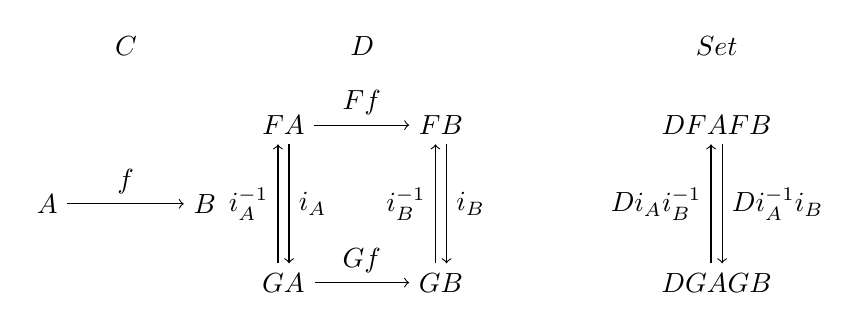
\begin{tikzpicture}[auto]
        \node (catc) at (0, 1) {$\cat{C}$};
        \node (A) at (-1, -1) {$A$};
        \node (B) at (1, -1) {$B$};
        \node (catd) at (3, 1) {$\cat{D}$};
        \node (FA) at (2, 0) {$FA$};
        \node (FB) at (4, 0) {$FB$};
        \node (GA) at (2, -2) {$GA$};
        \node (GB) at (4, -2) {$GB$};
        \node (catset) at (7.5, 1) {$\cat{Set}$};

        \node (FAFB) at (7.5, 0) {$\arset{D}{FA}{FB}$};
        \node (GAGB) at (7.5, -2) {$\arset{D}{GA}{GB}$};

        \draw[->] (A) to node{$f$}(B);
        \draw[->] (FA) to node{$Ff$}(FB);
        \draw[->] (GA) to node{$Gf$}(GB);
        \draw[->,transform canvas={xshift=2pt}] (FA) to node{$i_A$}(GA);
        \draw[->,transform canvas={xshift=2pt}] (FB) to node{$i_B$}(GB);
        \draw[->,transform canvas={xshift=-2pt}] (GA) to node{$i^{-1}_A$}(FA);
        \draw[->,transform canvas={xshift=-2pt}] (GB) to node{$i^{-1}_B$}(FB);
        \draw[->,transform canvas={xshift=2pt}] (FAFB) to node{$\arset{D}{i^{-1}_A}{i_B}$}(GAGB);
        \draw[->,transform canvas={xshift=-2pt}] (GAGB) to node{$\arset{D}{i_A}{i^{-1}_B}$}(FAFB);
      \end{tikzpicture}
    \end{center}
    次に$\arset{D}{FA}{FB}\cong\arset{D}{GA}{GB}$の$A,B$に対する自然性を証明する。\\
    すなわち、以下の図式が任意の射$\mor{g}{A'}{A},\ \mor{h}{B}{B'}$において可換になれば良い。
    \begin{center}
      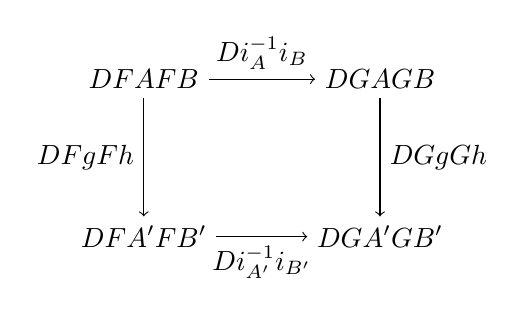
\begin{tikzpicture}[auto]
        \node (fab) at (0, 0) {$\arset{D}{FA}{FB}$};
        \node (gab) at (3, 0) {$\arset{D}{GA}{GB}$};
        \node (fab') at (0, -2) {$\arset{D}{FA'}{FB'}$};
        \node (gab') at (3, -2) {$\arset{D}{GA'}{GB'}$};

        \draw[->] (fab) to node{$\arset{D}{i^{-1}_A}{i_B}$}(gab);
        \draw[->] (fab') to node[swap]{$\arset{D}{i^{-1}_{A'}}{i_{B'}}$}(gab');
        \draw[->] (fab) to node[swap]{$\arset{D}{Fg}{Fh}$}(fab');
        \draw[->] (gab) to node{$\arset{D}{Gg}{Gh}$}(gab');
      \end{tikzpicture}
    \end{center}
    自然性の等式としては\[\arset{D}{Gg}{Gh}\circ\arset{D}{i^{-1}_A}{i_B} = \arset{D}{i^{-1}_{A'}}{i_{B'}}\circ \arset{D}{Fg}{Fh}\]のように書くことができ、射写像を合成して
    \[\arset{D}{i^{-1}_A\circ Gg}{Gh\circ i_B}=\arset{D}{Fg\circ i_{A'}^{-1}}{i_{B'}\circ Fh}\]が得られる。つまり二等式
    \[i^{-1}_A\circ Gg=Fg\circ i_{A'}^{-1},\ Gh\circ i_B=i_{B'}\circ Fh\]を示せばよい。しかしこれは自然変換$\nat{i}{F}{G},\ \nat{i^{-1}}{G}{F}$の自然性そのものであり成り立つ。よってが$\arset{D}{FA}{FB}\cong\arset{D}{GA}{GB}$の$A,B$に対して自然であることを示せた。
  \end{proof}
  心当たりがあるかもしれないが、今まで扱ってきた複数の対象において成り立つような同型のほとんどが自然同型である。次はこれらを例として確かめていく。
  \begin{prop}[$A\times 1\cong A$の自然性]
    $A\times 1\cong A$は$A$において自然である。
  \end{prop}
  \begin{proof}
    $A\times 1\cong A$の同型射はそれぞれ$\mor{\pi_{L,A\times 1}}{A\times 1}{A}$、$\mor{\tuple{id_A,!_A}}{A}{A\times 1}$であった。自然変換の始域と終域はそれぞれ恒等関手と積関手で表せそうである。

    実際に関手$\functor{Id_\cat{C}}{C}{C}$と$\functor{(-)\times 1}{C}{C}$の間の自然変換$\nat{\pi_L}{(-)\times 1}{Id_\cat{C}}$は任意の対象$A$に対して$(\pi_L)_A=\pi_{L,A\times 1}=\pi_A$と定義できる。自然同型の定義より、自然性を示すのは片方の自然変換だけで良いから、この$\pi_L$が自然性を満たすことを確かめる。
    \begin{align*}
      (\pi_L)_{B}\circ ((-)\times 1)(f)&=\pi_B\circ(f\times id_1)&\text{(自然変換と関手の定義)}\\
      &=\pi_B\circ\tuple{f\circ\pi_A,id_1\circ\pi_1}&\text{(射の積の定義)}\\
      &=f\circ\pi_A&\text{(積の普遍性)}\\
      &=Id(f)\circ(\pi_L)_A&\text{(自然変換と関手の定義)}
    \end{align*}
    よって$\pi_L$は自然変換であり、$A\times 1\cong A$は自然同型である。
    \begin{center}
      \begin{tikzpicture}[auto]
        \node (A) at (0, 0.75) {$A$};
        \node (B) at (1.5, 0.75) {$B$};
        \node (FA) at (3, 1.5) {$A\times 1$};
        \node (FB) at (4.5, 1.5) {$B\times 1$};
        \node (GA) at (3, 0) {$A$};
        \node (GB) at (4.5, 0) {$B$};

        \node (catc) at (0.75, 3) {$\cat{C}$};
        \node (catd) at (3.75, 3) {$\cat{C}$};

        \draw[->] (A) to node{$f$}(B);
        \draw[->] (FA) to node{$f\times id_1$}(FB);
        \draw[->] (GA) to node{$f$}(GB);
        \draw[->] (FA) to node{$\pi_A$}(GA);
        \draw[->] (FB) to node{$\pi_B$}(GB);

        \draw[->,bend left = 30] (catc) to node (funcf){$(-)\times 1$}(catd);
        \draw[->,bend right = 30] (catc) to node (funcg)[swap]{$Id_\cat{C}$}(catd);
        \draw[double,double equal sign distance,-implies,shorten >=5pt,shorten <=5pt] (funcf) -- node[label=right:$\pi_L$] {} (funcg);
      \end{tikzpicture}
    \end{center}

  \end{proof}
  \begin{prop}[$\arset{C}{X}{B}\cong\arset{C}{X}{B'}$の自然性]
    $B\cong B'\Longrightarrow \arset{C}{X}{B}\cong\arset{C}{X}{B'}$かつ$X$に対して自然。
  \end{prop}
  \begin{proof}[$\Longrightarrow$]
    $B\cong B'\Longrightarrow \arset{C}{X}{B}\cong\arset{C}{X}{B'}$はすでに示してあるので、同型射$\mor{\arset{C}{X}{i}}{\arset{C}{X}{B}}{\arset{Set}{X}{B'}}$が$X$に対して自然であることを示せば良い。\\
    任意の射$\mor{g}{Y}{X}$に対して、$\arset{C}{g}{B'}\circ\arset{C}{X}{i}=\arset{C}{Y}{i}\circ\arset{C}{g}{B}$が成り立つことを示せばよいが、双Hom関手の定義より\[\arset{C}{g}{i}=\arset{C}{g}{B'}\circ\arset{C}{X}{i}=\arset{C}{Y}{i}\circ\arset{C}{g}{B}\]が成り立つから明らかに自然である。
    \begin{center}
      \begin{tikzpicture}[auto]
        \node (A) at (-4, 5) {$X$};
        \node (B) at (-2, 5) {$Y$};
        \node (FA') at (0, 6) {$\arset{C}{X}{B}$};
        \node (FB') at (0, 4) {$\arset{C}{X}{B'}$};
        \node (GA') at (2, 6) {$\arset{C}{Y}{B}$};
        \node (GB') at (2, 4) {$\arset{C}{Y}{B'}$};

        \node (catc) at (-3, 8) {$\cat{C}$};
        \node (catd) at (1, 8) {$\cat{D}$};
  
        \draw[->] (A) to node{$i$}(B);

        \draw[->] (FA') to node{$\arset{C}{X}{i}$}(FB');
        \draw[->] (GA') to node{$\arset{C}{Y}{i}$}(GB');
        \draw[->] (FA') to node[swap]{$\arset{C}{g}{B}$}(GA');
        \draw[->] (FB') to node{$\arset{C}{g}{B'}$}(GB');
        \draw[->,bend left = 20] (catc) to node (funcf){$\arset{C}{-}{B}$}(catd);
        \draw[->,bend right = 20] (catc) to node (funcg)[swap]{$\arset{C}{-}{B'}$}(catd);
        \draw[double,double equal sign distance,-implies,shorten >=5pt,shorten <=5pt] (funcf) -- node[label=right:$\arset{C}{-}{i}$] {} (funcg);
      \end{tikzpicture}
    \end{center}
    この自然性が述べていることは、$\mor{f}{X}{B}$と対応する射$\mor{f'}{X}{B'}$、すなわち$f'=i\circ f,\ f=i^{-1}\circ f'$となる二射に対して、ある射$\mor{g}{Y}{X}$を両方に合成しても$f\circ g$と$f'\circ g$がまた対応することを示している。実際に計算すれば自明なことではあるが、射の前からの合成は射$f,f'$の対応関係を保つということが言える。
  \end{proof}
  \begin{proof}[$\Longleftarrow$]
    現在自然変換$\nat{\alpha}{\arset{C}{-}{B}}{\arset{C}{-}{B'}}$とその逆射$\nat{\alpha^{-1}}{\arset{C}{-}{B'}}{\arset{C}{-}{B}}$が与えられている。\\
    この二つの自然変換から$B$と$B'$の間の同型射を構成しなければ行けないが、$\alpha,\alpha^{-1}$の成分は射写像とは限らない。そのため少し工夫が必要になる。\\
    証明の方向性を示す。上の証明によると、$\mor{\arset{C}{X}{i}}{\arset{C}{X}{B}}{\arset{C}{X}{B'}}$が自然変換の$X$成分だった。この射から元の同型射である$i$を導出したい。ここでこの自然変換の$B$成分$\mor{\arset{C}{B}{i}}{\arset{C}{B}{B}}{\arset{C}{B}{B'}}$に恒等射$\mor{id_B}{B}{B}$を適用すると、射写像の定義より、$\arset{C}{B}{i}(id_B)=i$が成り立つ。\\
    これによって自然変換$\alpha,\alpha^{-1}$から元の同型射を取り出せば良い。\\
    $i=\alpha_B(id_B),\ i^{-1}=\alpha_{B'}^{-1}(id_B)$とし、$i,i^{-1}$が同型射になることを示す。$\alpha,\alpha^{-1}$の自然性より、\[\arset{C}{i^{-1}}{B'}\circ\alpha_B=\alpha_{B'}\circ\arset{C}{i^{-1}}{B}\]が成り立つ。両辺に恒等射$id_B$を適用して、
    \begin{align*}
      (\arset{C}{i^{-1}}{B'}\circ\alpha_B)id_B&=\arset{C}{i^{-1}}{B'}(i)&\text{($i$の定義)}\\
      &=i\circ i^{-1}&\text{(射写像の定義)}\\
      (\alpha_{B'}\circ\arset{C}{i^{-1}}{B})id_B&=\alpha_{B'}(i^{-1})&\text{(射写像の定義)}\\
      &=\alpha_{B'}(\alpha_{B'}^{-1}(id_B))&\text{($i^{-1}$の定義)}\\
      &=(\alpha_{B'}\circ\alpha_{B})(id_B)&\text{(写像の合成の定義)}\\
      &=id_{B'}
    \end{align*}
    よって$i\circ i^{-1}=id_{B'}$が示せた。同様に$i^{-1}\circ i=id_B$も成り立つため、$B\cong B'$が示せた。
  \end{proof}
  この証明のように、射集合が関わる自然変換の議論において恒等射が取れるように成分を指定する、というテクニックはよく使われている。この証明の核である$\arset{C}{B}{i}(id_B)=i$のより形式的な証明は、以前示した余評価射による恒等射の定義が用いられるので、興味があれば豊穣圏における弱米田の補題の証明あたりを読んでほしい。
  \begin{prop}[$\arset{C}{X}{A\times B}\cong \arset{C}{X}{A}\times \arset{C}{X}{B}$の自然性] \\
    $A\times B$が$A,B$における積対象$\iff\arset{C}{X}{A\times B}\cong \arset{C}{X}{A}\times \arset{C}{X}{B}$が$X$に対して自然
  \end{prop}
  \begin{prop}[$\arset{C}{X}{1}\cong I$の自然性] \\
    $1$が終対象$\iff\arset{C}{X}{1}\cong I$が$X$に対して自然
  \end{prop}
  \subsection{関手の合成の関手化}
  射の合成は$\cat{Set}$の射\[\mor{\circ}{\arset{C}{B}{C}\times\arset{C}{A}{B}}{\arset{C}{A}{C}}\]で表される。これは小さい圏の圏$\cat{Cat}$でも当てはまり、\[\mor{\circ}{\arset{Cat}{\cat{B}}{\cat{C}}\times\arset{Cat}{\cat{A}}{\cat{B}}}{\arset{Cat}{\cat{A}}{\cat{C}}}\]となる。しかし現在では関手の集合である射集合よりも関手を対象に持つ関手圏が定義できている。そこで関手の合成に現れる射集合を関手圏に置き換えることはできないだろうか。
  すなわち、\[\functor{\circ}{\funccat{B}{C}\times\funccat{A}{B}}{\funccat{A}{C}}\]となるような関手を考えたい。対象関数については単に関手の合成で表せるが、射関数をどのように構成するかがこれからの議論の核となる。
  \begin{define}[自然変換と関手の合成]
    関手$\functor{F,G}{C}{D}$と自然変換$\nat{\alpha}{F}{G}$、関手$\functor{F'}{D}{E}$に対して、自然変換$\nat{F'\circ\alpha}{F'F}{F'G}$を$\cat{C}$の任意の対象$C$に対して$(F'\circ\alpha)_C=F'(\alpha_C)$と定義する。\\
    すなわち、圏$\cat{D}$の$\alpha$の成分を関手$F$の射関数で圏$\cat{E}$に写す。そして得られた$F(\alpha_C)$を自然変換の成分とみなす、という流れである。さてこれが実際に自然変換となることを示そう。\\
    まず$F(\alpha_A)$が圏$\cat{C}$の任意の対象$C$に対して存在することは、$\alpha_A$がそうであることと、関手$F'$が任意の射を何かしらの射へ写すことから分かる。よって後は自然性を示せば良い。だがこれは関手$F'$の合成の保存と$\alpha$の自然性によって簡単に示せる。
    \[F'\alpha_B\circ F'Ff=F'(\alpha_B\circ Ff)=F'(Gf\circ\alpha_A)=F'Gf\circ F'\alpha_A\]よって確かに自然変換である。
    \begin{center}
      \begin{tikzpicture}[auto]
        \node (A) at (-4, 5) {$A$};
        \node (B) at (-2, 5) {$B$};
        \node (FA) at (-1, 6) {$FA$};
        \node (FB) at (1, 6) {$FB$};
        \node (GA) at (-1, 4) {$GA$};
        \node (GB) at (1, 4) {$GB$};
        \node (F'FA) at (2, 6) {$F'FA$};
        \node (F'FB) at (4, 6) {$F'FB$};
        \node (F'GA) at (2, 4) {$F'GA$};
        \node (F'GB) at (4, 4) {$F'GB$};
        \node (catc) at (-3, 8) {$\cat{C}$};
        \node (catd) at (0, 8) {$\cat{D}$};
        \node (cate) at (3, 8) {$\cat{E}$};

        \draw[->] (A) to node{$f$}(B);

        \draw[->] (FA) to node{$Ff$}(FB);
        \draw[->] (GA) to node{$Gf$}(GB);
        \draw[->] (FA) to node{$\alpha_A$}(GA);
        \draw[->] (FB) to node{$\alpha_B$}(GB);

        \draw[->] (F'FA) to node{$F'Ff$}(F'FB);
        \draw[->] (F'GA) to node{$F'Gf$}(F'GB);
        \draw[->] (F'FA) to node{$F'(\alpha_A)$}(F'GA);
        \draw[->] (F'FB) to node{$F'(\alpha_B)$}(F'GB);
        \draw[->] (catd) to node{$F'$}(cate);

        \draw[->,bend left = 20] (catc) to node (funcf){$F$}(catd);
        \draw[->,bend right = 20] (catc) to node (funcg)[swap]{$G$}(catd);
        \draw[double,double equal sign distance,-implies,shorten >=5pt,shorten <=5pt] (funcf) -- node[label=right:$\alpha$] {} (funcg);
      \end{tikzpicture}
    \end{center}
    \begin{center}
      \begin{tikzpicture}[auto]
        \node (A) at (-4, 5) {$A$};
        \node (B) at (-2, 5) {$B$};
        \node (F'FA) at (-1, 6) {$F'FA$};
        \node (F'FB) at (1, 6) {$F'FB$};
        \node (F'GA) at (-1, 4) {$F'GA$};
        \node (F'GB) at (1, 4) {$F'GB$};
        \node (catc) at (-3, 8) {$\cat{C}$};
        \node (cate) at (0, 8) {$\cat{E}$};

        \draw[->] (A) to node{$f$}(B);

        \draw[->] (F'FA) to node{$F'Ff$}(F'FB);
        \draw[->] (F'GA) to node{$F'Gf$}(F'GB);
        \draw[->] (F'FA) to node{$(F'\circ\alpha)_A$}(F'GA);
        \draw[->] (F'FB) to node{$(F'\circ\alpha)_B$}(F'GB);
        \draw[->,bend left = 20] (catc) to node (funcf){$F'F$}(catd);
        \draw[->,bend right = 20] (catc) to node (funcg)[swap]{$F'G$}(cate);
        \draw[double,double equal sign distance,-implies,shorten >=5pt,shorten <=5pt] (funcf) -- node[label=right:$F'\circ\alpha$] {} (funcg);
      \end{tikzpicture}
    \end{center}
  \end{define}
  次に自然変換の後ろに関手を合成する操作を考えよう。
  \begin{define}[関手と自然変換の合成]
    関手$\functor{F',G'}{D}{E}$と自然変換$\nat{\beta}{F'}{G'}$、関手$\functor{F}{C}{D}$に対して自然変換$\nat{\beta\circ F}{F'F}{G'F}$を$\cat{C}$の任意の対象$C$に対して$(\beta\circ F)_C=\beta_{FC}$と定義する。これは自然変換$\beta$の量化の範囲を$F$で写された範囲に限定するという流れである。\\
    ここでの$\mor{\beta_{FC}}{F'FC}{G'FC}$は単に$\beta$の$FC$成分であるから自然性はすでに満たす。圏$\cat{C}$の任意の対象$C$に対して成分$\beta_{FC}$が存在するかどうかであるが、関手$F$は$C$を何らかの対象に写すため、$\beta_{FC}$は存在する。よって$\beta F$は自然変換である。
    \begin{center}
      \begin{tikzpicture}[auto]
        \node (A) at (-4, 5) {$A$};
        \node (B) at (-2, 5) {$B$};
        \node (FA) at (-1, 5) {$FA$};
        \node (FB) at (1, 5) {$FB$};
        \node (F'FA) at (2, 6) {$F'FA$};
        \node (F'FB) at (4, 6) {$F'FB$};
        \node (F'GA) at (2, 4) {$G'FA$};
        \node (F'GB) at (4, 4) {$G'FB$};
        \node (catc) at (-3, 8) {$\cat{C}$};
        \node (catd) at (0, 8) {$\cat{D}$};
        \node (cate) at (3, 8) {$\cat{E}$};

        \draw[->] (A) to node{$f$}(B);

        \draw[->] (FA) to node{$Ff$}(FB);

        \draw[->] (F'FA) to node{$F'Ff$}(F'FB);
        \draw[->] (F'GA) to node{$G'Ff$}(F'GB);
        \draw[->] (F'FA) to node{$\beta_{FA}$}(F'GA);
        \draw[->] (F'FB) to node{$\beta_{FB}$}(F'GB);
        \draw[->] (catc) to node{$F$}(catd);

        \draw[->,bend left = 20] (catd) to node (funcf){$F'$}(cate);
        \draw[->,bend right = 20] (catd) to node (funcg)[swap]{$G'$}(cate);
        \draw[double,double equal sign distance,-implies,shorten >=5pt,shorten <=5pt] (funcf) -- node[label=right:$\beta$] {} (funcg);
      \end{tikzpicture}
    \end{center}

    \begin{center}
      \begin{tikzpicture}[auto]
        \node (A) at (-4, 5) {$A$};
        \node (B) at (-2, 5) {$B$};
        \node (F'FA) at (-1, 6) {$F'FA$};
        \node (F'FB) at (1, 6) {$F'FB$};
        \node (F'GA) at (-1, 4) {$G'FA$};
        \node (F'GB) at (1, 4) {$G'FB$};
        \node (catc) at (-3, 8) {$\cat{C}$};
        \node (cate) at (0, 8) {$\cat{E}$};
  
        \draw[->] (A) to node{$f$}(B);
  
        \draw[->] (F'FA) to node{$F'Ff$}(F'FB);
        \draw[->] (F'GA) to node{$G'Ff$}(F'GB);
        \draw[->] (F'FA) to node{$(\beta\circ F)_A$}(F'GA);
        \draw[->] (F'FB) to node{$(\beta\circ F)_B$}(F'GB);
  
        \draw[->,bend left = 20] (catc) to node (funcf){$F'F$}(cate);
        \draw[->,bend right = 20] (catc) to node (funcg)[swap]{$G'F$}(cate);
        \draw[double,double equal sign distance,-implies,shorten >=5pt,shorten <=5pt] (funcf) -- node[label=right:$\beta\circ F$] {} (funcg);
      \end{tikzpicture}
    \end{center}
  \end{define}
  次にいよいよ合成を行う関手の射関数となるような操作を定義する。またこの合成は関手圏における射の合成である垂直合成と区別するため水平合成と呼ぶことにする。
  \begin{define}[自然変換の水平合成]
    関手$\functor{F,G}{C}{D},\ \functor{F',G'}{D}{E}$と自然変換$\nat{\alpha}{F}{G},\ \nat{\beta}{F'}{G'}$に対して\textbf{垂直合成}された自然変換$\nat{\beta\alpha}{F'F}{G'G}$を\[\beta\circ\alpha = \alpha G'\cdot F\beta = G\beta\cdot\alpha F'\]とする。\\
    \begin{center}
      \begin{tikzpicture}[auto]
        \node (cat) at (1, 1) {$\funccat{C}{E}$};
        \node (FF) at (0, 0) {$F'F$};
        \node (FG) at (2, 0) {$F'G$};
        \node (GF) at (0, -2) {$G'F$};
        \node (GG) at (2, -2) {$G'G$};
        \draw[double,double equal sign distance,-implies] (FF) to node{$\beta\circ F$}(GF);
        \draw[double,double equal sign distance,-implies] (FG) to node{$\beta\circ G$}(GG);
        \draw[double,double equal sign distance,-implies] (FF) to node{$F'\circ\alpha$}(FG);
        \draw[double,double equal sign distance,-implies] (GF) to node{$G'\circ\beta$}(GG);
      \end{tikzpicture}
    \end{center}
    成分を見ると、$\cat{C}$の任意の対象$C$に対して成分\[(\beta\circ\alpha)_C=G'\alpha_C\circ \beta_{FC}=\beta_{GC}\circ F'\alpha_C\]となる。
    自然変換と関手の合成と関手の自然変換の合成をそれぞれ用いて定義されているが、これらが自然変換であることはすでに示した。よってその二つを合成した$\beta\circ\alpha$も自然変換である。\\
    さて自然変換の水平合成の直感を得るためにも$\alpha G'\cdot F\beta = G\beta\cdot\alpha F'$を示そう。これは上に書いたように$A$に対して成分の等式\[G'\alpha_A\circ \beta_{FA}=\beta_{GA}\circ F'\alpha_A\]が成り立てば良い。
    \begin{center}
      \begin{tikzpicture}[auto]
        \node (A) at (-2, 5) {$A$};
        \node (FA) at (0, 6) {$FA$};
        \node (GA) at (0, 4) {$GA$};
        \node (F'FA) at (2, 6) {$F'FA$};
        \node (F'FB) at (4, 6) {$G'FA$};
        \node (F'GA) at (2, 4) {$F'GA$};
        \node (F'GB) at (4, 4) {$G'GA$};
        \node (catc) at (-2, 8) {$\cat{C}$};
        \node (catd) at (0, 8) {$\cat{D}$};
        \node (cate) at (3, 8) {$\cat{E}$};


        \draw[->] (FA) to node{$\alpha_A$}(GA);

        \draw[->] (F'FA) to node{$\beta_{FA}$}(F'FB);
        \draw[->] (F'GA) to node{$\beta_{GA}$}(F'GB);
        \draw[->] (F'FA) to node{$F'\alpha_A$}(F'GA);
        \draw[->] (F'FB) to node{$G'\alpha_A$}(F'GB);


        \draw[->,bend left = 20] (catd) to node (funcf'){$F'$}(cate);
        \draw[->,bend right = 20] (catd) to node (funcg')[swap]{$G'$}(cate);
        \draw[->,bend left = 30] (catc) to node (funcf){$F$}(catd);
        \draw[->,bend right =30] (catc) to node (funcg)[swap]{$G$}(catd);
        \draw[double,double equal sign distance,-implies,shorten >=5pt,shorten <=5pt] (funcf) -- node[label=right:$\alpha$] {} (funcg);
        \draw[double,double equal sign distance,-implies,shorten >=5pt,shorten <=5pt] (funcf') -- node[label=right:$\beta$] {} (funcg');
      \end{tikzpicture}
    \end{center}
    ここで$FA=B,\ GA=C, \alpha_A=f$と置くと、これは明らかに$\beta$の自然性であり成り立つ。
    \begin{center}
      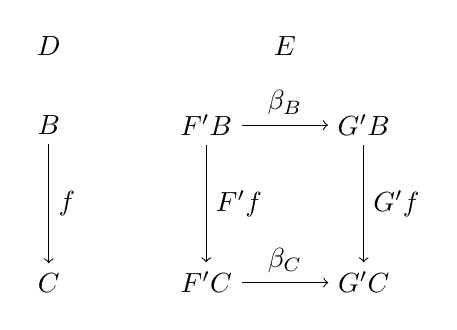
\begin{tikzpicture}[auto]
        \node (FA) at (0, 6) {$B$};
        \node (GA) at (0, 4) {$C$};
        \node (F'FA) at (2, 6) {$F'B$};
        \node (F'FB) at (4, 6) {$G'B$};
        \node (F'GA) at (2, 4) {$F'C$};
        \node (F'GB) at (4, 4) {$G'C$};
        \node (catd) at (0, 7) {$\cat{D}$};
        \node (cate) at (3, 7) {$\cat{E}$};
        \draw[->] (FA) to node{$f$}(GA);

        \draw[->] (F'FA) to node{$\beta_{B}$}(F'FB);
        \draw[->] (F'GA) to node{$\beta_{C}$}(F'GB);
        \draw[->] (F'FA) to node{$F'f$}(F'GA);
        \draw[->] (F'FB) to node{$G'f$}(F'GB);
      \end{tikzpicture}
    \end{center}
  \end{define}
  また、$\alpha$を恒等自然変換とすると関手と自然変換の合成になり、$\beta$を恒等自然変換とすると自然変換と関手の合成になる。よってどちらも自然変換の水平合成と呼ぶことにする。
  \begin{define}[関手を合成する関手]
    関手を合成する関手$\functor{\circ}{\funccat{D}{E}\times \funccat{C}{D}}{\funccat{C}{E}}$を以下のように定義する。
    \begin{quote}
			\begin{mydescription}
		\item[対象関数]対象関数
    \[\functor{\circ}{\obj{\funccat{D}{E}\times\funccat{C}{D}}}{\obj{\funccat{C}{E}}}\]は、積圏の対象の集合の定義より、\[\functor{\circ}{\obj{\funccat{D}{E}}\times\obj{\funccat{C}{D}}}{\obj{\funccat{C}{E}}}\]と表せる。また関手圏の対象集合の定義より、\[\mor{\circ}{\arset{Cat}{\cat{D}}{\cat{E}}\times\arset{Cat}{\cat{C}}{\cat{D}}}{\arset{Cat}{\cat{C}}{\cat{E}}}\]とも表せるから、$\cat{Cat}$の定義に用いられる関手の合成を対象関数とする。
		\item[射関数]任意の関手$\functor{F,G}{C}{D},\ \functor{F',G'}{D}{E}$に対する射関数\[\mor{\circ}{\arset{\funccat{D}{E}\times\funccat{C}{D}}{\tuple{F',F}}{\tuple{G',G}}}{\arset{\funccat{C}{E}}{F'\circ F}{G'\circ G}}\]を任意の自然変換$\nat{\alpha}{F}{G},\ \nat{\beta}{F'}{G'}$に対して
    \[\circ(\beta,\alpha)=\beta\circ\alpha\]と定義する。
    \begin{center}
      \begin{tikzpicture}[auto]
        \node (cata) at (0, 1) {$\funccat{D}{E}\times\funccat{C}{D}$};
        \node (cata) at (2, 1) {$\funccat{C}{E}$};
        \node (F'F) at (0, 0) {$\tuple{F',F}$};
        \node (G'G) at (0, -2) {$\tuple{G',G}$};
        \draw[->] (F'F) to node{$\tuple{\beta,\alpha}$}(G'G);
        \node (F'cF) at (2, 0) {$F'\circ F$};
        \node (G'cG) at (2, -2) {$G'\circ G$};
        \draw[double,double equal sign distance,-implies] (F'cF) to node{$\beta\circ\alpha$}(G'cG);
        \draw[-,dashed] (F'F) to (F'cF);
        \draw[-,dashed] (G'G) to (G'cG);

      \end{tikzpicture}
    \end{center}
		\item[恒等射の保存]積圏の恒等射の定義より、$\tuple{F',F}$の恒等射は$\nat{\tuple{ID_{F'},ID_{F}}}{\tuple{F',F}}{\tuple{F',F}}$であるから、$ID_{F'}\circ ID_{F}=ID_{F'F}$を示せば良い。これは$\cat{C}$の任意の対象$C$おいて
    \begin{align*}
      (ID_{F'}\circ ID_F)_C &= F'(ID_{F})_C\circ (ID_{F'})_{FC}&\text{(自然変換の水平合成)}\\
      &=F'(id_{FC})\circ id_{F'FC}&\text{(恒等自然変換の定義)}\\
      &=id_{F'FC}\circ id_{F'FC}&\text{(関手の恒等射の保存)}\\
      &=id_{F'FC}
    \end{align*}
    となるから$ID_{F'}\circ ID_{F}=ID_{F'F}$である。
		\item[射の合成の保存]任意の$\functor{F,G,H}{C}{D},\ \functor{F',G',H'}{D}{E}$と自然変換$\nat{\alpha}{F}{G},\ \nat{\beta}{F'}{G'},\ \nat{\alpha'}{G}{H},\ \nat{\beta'}{G'}{H'}$に対して
    \[(\beta'\cdot\beta)\circ(\alpha'\cdot\alpha)=(\beta'\circ\alpha')\cdot(\beta\circ\alpha)\]が成り立つことを示せば良い。
    \begin{center}
      \begin{tikzpicture}[auto]
        \node (catc) at (-3, 8) {$\cat{C}$};
        \node (catd) at (0, 8) {$\cat{D}$};
        \node (cate) at (3, 8) {$\cat{E}$};
        \draw[->,bend left = 40] (catd) to node (funcf'){$F'$}(cate);
        \draw[->] (catd) to node[yshift =-7,fill=white] (funcg'){$G'$}(cate);
        \draw[->,bend right = 40] (catd) to node (funch')[swap]{$H'$}(cate);

        \draw[->,bend left = 40] (catc) to node (funcf){$F$}(catd);
        \draw[->] (catc) to node[yshift =-7,fill=white] (funcg){$G$}(catd);
        \draw[->,bend right =40] (catc) to node (funch)[swap]{$H$}(catd);
        \draw[double,double equal sign distance,-implies,shorten >=0pt,shorten <=2pt] (funcf) -- node[label=right:$\alpha$] {} (funcg);
        \draw[double,double equal sign distance,-implies,shorten >=0pt,shorten <=2pt] (funcf') -- node[label=right:$\beta$] {} (funcg');
        \draw[double,double equal sign distance,-implies,shorten >=2pt,shorten <=0pt] (funcg) -- node[label=right:$\alpha'$] {} (funch);
        \draw[double,double equal sign distance,-implies,shorten >=2pt,shorten <=0pt] (funcg') -- node[label=right:$\beta'$] {} (funch');
      \end{tikzpicture}
    \end{center}
		圏$\cat{C}$の任意の対象$A$に対して、
    \begin{align*}
      ((\beta'\cdot\beta)\circ(\alpha'\cdot\alpha))_A&=H'(\alpha'\cdot\alpha)_A\circ(\beta'\cdot\beta)_{FA}&\text{(水平合成の定義)}\\
      &=H'\alpha'_A\circ H'\alpha_A\circ\beta'_{FA}\circ\beta_{FA}&\text{(垂直合成の定義)}\\
      &=H'\alpha'_A\circ\beta'_{GA}\circ G'\alpha_A\circ\beta_{FA}&\text{($\beta$の自然性)}\\
      &=(\beta'\circ\alpha')_A\circ(\beta\circ\alpha)_A&\text{(水平合成の定義)}\\
      &=((\beta'\circ\alpha')\cdot(\beta\circ\alpha))_A&\text{(垂直合成の定義)}
    \end{align*}
    \begin{center}
      \begin{tikzpicture}[auto]
        \node (cata) at (0, 1) {$\funccat{D}{E}\times\funccat{C}{D}$};
        \node (cata) at (2, 1) {$\funccat{C}{E}$};
        \node (F'F) at (0, 0) {$\tuple{F',F}$};
        \node (G'G) at (0, -2) {$\tuple{G',G}$};
        \node (H'H) at (0, -4) {$\tuple{H',H}$};

        \draw[->] (F'F) to node[swap]{$\tuple{\beta,\alpha}$}(G'G);
        \draw[->] (G'G) to node[swap]{$\tuple{\beta',\alpha'}$}(H'H);

        \node (F'cF) at (2, 0) {$F'\circ F$};
        \node (G'cG) at (2, -2) {$G'\circ G$};
        \node (H'cH) at (2, -4) {$H'\circ H$};

        \draw[double,double equal sign distance,-implies] (F'cF) to node[swap]{$\beta\circ\alpha$}(G'cG);
        \draw[double,double equal sign distance,-implies] (G'cG) to node[swap]{$\beta'\circ\alpha'$}(H'cH);
        \draw[double,double equal sign distance,-implies,bend left = 30] (F'cF) to node{$(\beta'\cdot\beta)\circ(\alpha'\cdot\alpha)$}(H'cH);
        \draw[-,dashed] (F'F) to (F'cF);
        \draw[-,dashed] (G'G) to (G'cG);
        \draw[-,dashed] (H'H) to (H'cH);

      \end{tikzpicture}
    \end{center}
    よって$(\beta'\cdot\beta)\circ(\alpha'\cdot\alpha)=(\beta'\circ\alpha')\cdot(\beta\circ\alpha)$である。またこの性質を相互交換法則と呼ぶことにする。
		\end{mydescription}
		\end{quote}
  \end{define}
  関手の合成を関手として定義できたわけだが、これを$\cat{Cat}$における射の合成の代わりに使用できるかと考えるが、それを行うには圏の定義から考え直さなくてはいけなくなる。現時点で触れる予定は無いが、興味がある場合は2-Categoryに関する文献を読むと良い。\\
  また関手の同型の保存より以下の命題がすぐに成り立つ。
  \begin{prop}[関手合成の同型の保存]
    関手$\functor{F,F'}{C}{D},\ \functor{G,G'}{D}{E}$に対して$F\cong F',\ G\cong G'\Longrightarrow G\circ F\cong G'\circ F'$
  \end{prop}
  \begin{proof}
    双関手の同型の保存より\[F\cong F',\ G\cong G'\Longrightarrow\tuple{G,F}\cong\tuple{G',F'}\]\\
    また関手を合成する関手の同型の保存より、\[\tuple{G,F}\cong\tuple{G',F'}\Longrightarrow G\circ F\cong G'\circ F'\]
    よって$F\cong F',\ G\cong G'\Longrightarrow G\circ F\cong G'\circ F'$が成り立つ。
  \end{proof}
  さて、自然変換の水平合成や相互交換法則に触れた理由として、関手圏やその合成を行う関手の性質によって、関手や自然変換の満たすべき性質を復元できるからである。特に関手の合成の保存や、自然性などは仮定する動機が不十分であったから、これらを$\cat{Cat}$の持つ性質と見なして改めて導出しよう。\\


    自然性と水平合成の関係を見る。一点離散圏$\cat{1}$と任意の圏$\cat{C,D}$、関手$\functor{A,B}{1}{C},\ \functor{F,G}{C}{D}$、自然変換$\nat{f}{A}{B},\ \nat{\alpha}{F}{G}$を考える。
    \begin{center}
      \begin{tikzpicture}[auto]
        \node (*) at (-2, 5) {$*$};
        \node (A) at (0, 6) {$A*$};
        \node (B) at (0, 4) {$B*$};
        \node (FA) at (2, 6) {$FA*$};
        \node (GA) at (4, 6) {$GA*$};
        \node (FB) at (2, 4) {$FB*$};
        \node (GB) at (4, 4) {$GB*$};
        \node (cat1) at (-2, 8) {$\cat{1}$};
        \node (catc) at (0, 8) {$\cat{C}$};
        \node (catd) at (3, 8) {$\cat{D}$};


        \draw[->] (A) to node{$f_*$}(B);

        \draw[->] (F'FA) to node{$\alpha_{A*}$}(F'FB);
        \draw[->] (F'GA) to node{$\alpha_{B*}$}(F'GB);
        \draw[->] (F'FA) to node{$Ff_*$}(F'GA);
        \draw[->] (F'FB) to node{$Gf_*$}(F'GB);

        \draw[->,bend left = 30] (cat1) to node (funcf'){$A$}(catc);
        \draw[->,bend right = 30] (cat1) to node (funcg')[swap]{$B$}(catc);
        \draw[->,bend left = 20] (catc) to node (funcf){$F$}(catd);
        \draw[->,bend right =20] (catc) to node (funcg)[swap]{$G$}(catd);
        \draw[double,double equal sign distance,-implies,shorten >=5pt,shorten <=5pt] (funcf) -- node[label=right:$\alpha$] {} (funcg);
        \draw[double,double equal sign distance,-implies,shorten >=5pt,shorten <=5pt] (funcf') -- node[label=right:$f$] {} (funcg');
      \end{tikzpicture}
    \end{center}
    $A=A(*),\ B=B(*),\ f=f_*$とすると、以下のような図式が書ける。
    \begin{center}
      \begin{tikzpicture}[auto]
        \node (*) at (-2, 5) {$*$};
        \node (A) at (0, 6) {$A$};
        \node (B) at (0, 4) {$B$};
        \node (FA) at (2, 6) {$FA$};
        \node (GA) at (4, 6) {$GA$};
        \node (FB) at (2, 4) {$FB$};
        \node (GB) at (4, 4) {$GB$};
        \node (cat1) at (-2, 8) {$\cat{1}$};
        \node (catc) at (0, 8) {$\cat{C}$};
        \node (catd) at (3, 8) {$\cat{D}$};


        \draw[->] (A) to node{$f$}(B);

        \draw[->] (F'FA) to node{$\alpha_A$}(F'FB);
        \draw[->] (F'GA) to node{$\alpha_B$}(F'GB);
        \draw[->] (F'FA) to node{$Ff$}(F'GA);
        \draw[->] (F'FB) to node{$Gf$}(F'GB);


        \draw[->,bend left = 30] (cat1) to node (funcf'){$A$}(catc);
        \draw[->,bend right = 30] (cat1) to node (funcg')[swap]{$B$}(catc);
        \draw[->,bend left = 20] (catc) to node (funcf){$F$}(catd);
        \draw[->,bend right =20] (catc) to node (funcg)[swap]{$G$}(catd);
        \draw[double,double equal sign distance,-implies,shorten >=5pt,shorten <=5pt] (funcf) -- node[label=right:$\alpha$] {} (funcg);
        \draw[double,double equal sign distance,-implies,shorten >=5pt,shorten <=5pt] (funcf') -- node[label=right:$f$] {} (funcg');
      \end{tikzpicture}
    \end{center}
    これは任意の射、任意の対象で成り立つから、明らかに自然変換の図式である。\\

    関手の合成の保存と相互交換法則の関係性を見る。一点離散圏$\cat{1}$と任意の圏$\cat{C,D}$、関手$\functor{A,B,C}{1}{C},\ \functor{F}{C}{D}$、自然変換$\nat{f}{A}{B},\ \nat{g}{B}{C}$を考えると、相互交換法則より\[(ID_F\cdot ID_F)\circ(g\cdot f)=(ID_F\circ g)\cdot(ID_F\circ f)\]が成り立つ。この自然変換の$*$成分を取ると、
    \begin{align*}
      ((ID_F\cdot ID_F)\circ(g\cdot f))_*&=F(g\cdot f)_*\circ(ID_F\cdot ID_F)_{C*}&\text{(水平合成の定義)}\\
      &=F(g\cdot f)_*&\text{(恒等自然変換の定義)}\\
      ((ID_F\circ g)\cdot(ID_F\circ f))_*&=(ID_F\circ g)_*\circ(ID_F\circ f)_*&\text{(垂直合成の定義)}\\
      &=Fg_*\circ Ff_*&\text{(水平合成の定義)}\\
    \end{align*}
    となり、$f_*=f,\ g_*=g$とすると、$(g\cdot f)_*=g\circ f$であるから、
    この等式は$F(g\circ f)=Fg\circ Ff$と変形できる。
    \begin{center}
      \begin{tikzpicture}[auto]
        \node (catc) at (-3, 8) {$\cat{1}$};
        \node (catd) at (0, 8) {$\cat{C}$};
        \node (cate) at (3, 8) {$\cat{D}$};
        \draw[->,bend left = 40] (catd) to node (funcf'){$F$}(cate);
        \draw[->] (catd) to node[yshift =-7,fill=white] (funcg'){$F$}(cate);
        \draw[->,bend right = 40] (catd) to node (funch')[swap]{$F$}(cate);

        \draw[->,bend left = 40] (catc) to node (funcf){$A$}(catd);
        \draw[->] (catc) to node[yshift =-7,fill=white] (funcg){$B$}(catd);
        \draw[->,bend right =40] (catc) to node (funch)[swap]{$C$}(catd);
        \draw[double,double equal sign distance,-implies,shorten >=0pt,shorten <=2pt] (funcf) -- node[label=right:$f$] {} (funcg);
        \draw[double,double equal sign distance,-implies,shorten >=0pt,shorten <=2pt] (funcf') -- node[label=right:$ID_F$] {} (funcg');
        \draw[double,double equal sign distance,-implies,shorten >=2pt,shorten <=0pt] (funcg) -- node[label=right:$g$] {} (funch);
        \draw[double,double equal sign distance,-implies,shorten >=2pt,shorten <=0pt] (funcg') -- node[label=right:$ID_F$] {} (funch');
    \end{tikzpicture}
  \end{center}
  \subsection{圏同値}
  圏$\cat{C,D}$の同型であるためには、2つの関手$\functor{F}{C}{D},\ \functor{G}{D}{C}$が$F\circ G=Id_D,\ G\circ F=Id_C$とならなければならない。ここで圏$\cat{C,D}$のある対象$C,D$を適用すると、$FG(D)=D,\ GF(C)=C$となる。これまでの議論で気がついたかもしれないが、圏論には二つの対象が等しいことを示す手段がない。そのため圏が同型であることを示すのは難しい。対象の等価性についてはこれまで同型を使用してきたから、これらの等号を同型に一般化することを考えよう。\\
  \begin{define}
    圏$C,D$に対してある二関手$\functor{F}{C}{D},\ \functor{G}{D}{C}$が存在して$F\circ G\cong Id_D,\ G\circ F\cong Id_C$となるとき、$\cat{C,D}$は\textbf{圏同値}であるといい、$\cat{C}\simeq \cat{D}$と表記する。また$F,G$を\textbf{同値関手}と呼ぶことにする。
  \end{define}
  \begin{prop}[圏同値の同値性]
    圏同値$\cat{C}\simeq \cat{D}$は同値関係である。
  \end{prop}
  \begin{proof}
    \begin{quote}~\\
			\begin{mydescription}
				\item[反射律] $\cat{C}\simeq \cat{C}$を示せば良い。同値関手を$Id_\cat{C},Id_\cat{C}$とすると、$Id_\cat{C}\circ Id_\cat{C}=Id_\cat{C}$である。$Id_\cat{C}\circ Id_\cat{C}$と$Id_\cat{C}$が等しいから、同型の反射律より$Id_\cat{C}\circ Id_\cat{C}\cong Id_\cat{C}$が成り立つ。
				\item[対称律]定義の対称性より自明
				\item[推移律]$\cat{C}\simeq \cat{D},\ \cat{D}\simeq\cat{E}\Longrightarrow \cat{C}\simeq\cat{E}$を示せばよい。それぞれの同値関手を$\functor{F}{C}{D},\ \functor{G}{D}{C},\ \functor{F'}{D}{E},\ \functor{G'}{E}{D}$とする。この時、
				\[GF\cong Id_\cat{C},\ FG\cong Id_\cat{D}\]
        \[G'F'\cong Id_\cat{D},\ F'G'\cong Id_\cat{E}\]が成り立つから、ここから\[GG'F'F\cong Id_\cat{C},\ F'FGG'\cong Id_\cat{E}\]を示せばよい。\\
        \begin{align*}
          G'F'&\cong Id_D\\
          G'F'F&\cong F&\text{(関手合成の同型の保存)}\\
          GG'F'F&\cong GF&\text{(関手合成の同型の保存)}\\
          GG'F'F&\cong Id_E&\text{(同型の推移律)}
        \end{align*}
        同様に$F'FGG'\cong Id_\cat{E}$も成り立つから、確かに$\cat{C}\simeq\cat{E}$である。
      \end{mydescription}
    \end{quote}
  \end{proof}
  ここまでで様々な概念の等価性について議論してきたが、それらが一段落ついたため一度整理しようと思う。
  \begin{table}[htb]
    \centering
      \begin{tabular}{|c||c|c|c|}  \hline
      &圏$\cat{C,D}$&関手$F,G$&自然変換$\alpha,\beta$\\ \hline \hline
      同一&$\cat{C}=\cat{D}$&$F=G$&$\alpha=\beta$\\ \hline
      同型&$\cat{C}\cong\cat{D}$&$F\cong G$&\\ \hline
      同値&$\cat{C}\simeq\cat{D}$&&\\ \hline
    \end{tabular}
  \end{table}
  上の表は行が各概念の等価性を表していて、列が比較する対象を示している。意識すべきことはある二概念の等価性、例えば$\cat{C}\cong \cat{D}$はその右上の等価性$F=G$によって表される。これはすべての欄に当てはまっていて、例えば圏同値\[\cat{C}\simeq\cat{D}\]は関手の同型である自然同型\[FG\cong Id_\cat{D},\ GF\cong Id_\cat{C}\]によって定義されていて、この関手の同型は自然変換の等号\[i\circ i^{-1}=ID_{FG},\ i^{-1}\circ i=ID_{Id_\cat{D}}\]で定義される。\\
  この表に関手の同値性が存在しないのは、右上の自然変換の同型が存在しないからである。もし自然変換の同型を考えるのであれば、自然変換と自然変換の間の射が存在し、それの同一性を示すことが可能である必要がある。しかし自然変換は圏の射によって構成されいて、自然変換と自然変換の間の射が存在するとしたらそれは圏の射と射の間の射が必要になってしまう。\\
  また、$\cat{Cat}$においてはある圏$\cat{C}$の対象は関手$\functor{A}{1}{C}$で、射は$\natf{f}{A}{B}{1}{C}$で表せるのだった。そのため一般の圏$\cat{C}$での等価性を考えるのであれば、表の右上を切り取れば良い。
  \begin{table}[htb]
    \centering
      \begin{tabular}{|c||c|c|}  \hline
      &対象$A,B$&射$f,g$\\ \hline \hline
      同一&$A=B$&$f=g$\\ \hline
      同型&$A\cong B$&\\ \hline
    \end{tabular}
  \end{table}

  さて圏同値の話に戻るが、この圏同値の例として一点離散圏の普遍性を自然同型によって弱めてみよう。
  \begin{define}
    ある圏$\cat{I}$は任意の圏$\cat{X}$に対してある関手$\functor{I_\cat{X}}{X}{I}$が存在して、任意の関手$\functor{F}{X}{I}$に対し$I_X\cong F$が成り立つとする。
  \end{define}
  一点離散圏の普遍性では二つの関手の同型$I_X\cong F$ではなく、関手の同一性$I_X=F$が成り立つような性質であったことを思い出してほしい。そういった意味で一点離散圏の普遍性の一般化と言える。\\
  次にこの圏がどのような対象や射を持つかを調べよう。圏同型$\cat{C}\cong\funccat{1}{C}$により圏$\cat{I}$の任意の対象は関手$\functor{A}{1}{I}$で表せる。ところが圏$\cat{I}$の性質により、ある関手$\functor{I_\cat{1}}{1}{I}$と同型$A\cong I_\cat{1}$になる。すなわち圏
	\subsection{エンド}
  定自然変換$\natf{\varDelta f}{\varDelta A}{\varDelta B}{C}{D}$は、圏$\cat{C}$の任意の対象$C$に対して$(\varDelta f)_C=f$となる自然変換であった。一方で定関手$\varDelta A$でも$\varDelta A(C)=A$が成り立つが、この性質は定写像$\mor{\varDelta A}{\obj{C}}{\obj{D}}$によって定義されている。定自然変換と違い、関手に対象を適用する操作は対象関数で与えられているが、自然変換には与えられておらず、自然変換の成分を取る操作は写像によって定義したわけではない。\\
  自然変換を対象によって添え字付けられた射の束、と定義するのでは無く、射集合の何らかの操作によって定義できると考えたかもしれない。これは実際にエンドと呼ばれる一種の普遍性を用いることで、自然変換を再定義することができる。\\
  \begin{prop}[自然変換の普遍性]
    圏$\cat{C}$の任意の対象$C$に対して$\cat{Set}$の射$\mor{\lambda_C}{\arset{\funccat{C}{D}}{F}{G}}{\arset{D}{FC}{GC}}$が存在し、$\cat{C}$の任意の射$\mor{f}{A}{B}$に対して、\[\arset{D}{FA}{Gf}\circ\lambda_A=\arset{D}{Ff}{GB}\circ\lambda_B\]を満たす。
    
    \begin{center}
      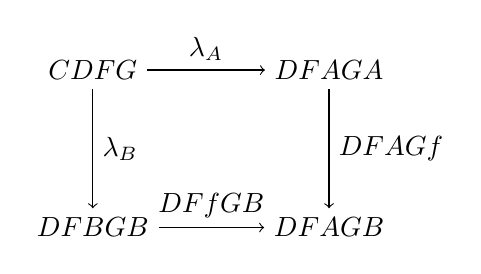
\begin{tikzpicture}[auto]
        \node (FG) at (0, 0) {$\arset{\funccat{C}{D}}{F}{G}$};
        \node (FAGA) at (3, 0) {$\arset{D}{FA}{GA}$};
        \node (FBGB) at (0, -2) {$\arset{D}{FB}{GB}$};
        \node (FAGB) at (3, -2) {$\arset{D}{FA}{GB}$};

        \draw[->] (FG) to node{$\lambda_A$}(FAGA);
        \draw[->] (FG) to node{$\lambda_B$}(FBGB);
        \draw[->] (FAGA) to node{$\arset{D}{FA}{Gf}$}(FAGB);
        \draw[->] (FBGB) to node{$\arset{D}{Ff}{GB}$}(FAGB);

      \end{tikzpicture}
    \end{center}
    
    またある対象$X$に対しても任意の対象$C$に対する$\mor{\mu_C}{\arset{\funccat{C}{D}}{F}{G}}{\arset{D}{FC}{GC}}$が存在し、\[\arset{D}{FA}{Gf}\circ\mu_A=\arset{D}{Ff}{GB}\circ\mu_B\]を満たすのであれば、
    \begin{center}
      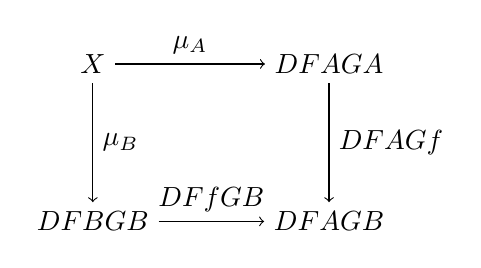
\begin{tikzpicture}[auto]
        \node (FG) at (0, 0) {$X$};
        \node (FAGA) at (3, 0) {$\arset{D}{FA}{GA}$};
        \node (FBGB) at (0, -2) {$\arset{D}{FB}{GB}$};
        \node (FAGB) at (3, -2) {$\arset{D}{FA}{GB}$};

        \draw[->] (FG) to node{$\mu_A$}(FAGA);
        \draw[->] (FG) to node{$\mu_B$}(FBGB);
        \draw[->] (FAGA) to node{$\arset{D}{FA}{Gf}$}(FAGB);
        \draw[->] (FBGB) to node{$\arset{D}{Ff}{GB}$}(FAGB);

      \end{tikzpicture}
    \end{center}
    任意の対象$C$に対して$\mu_C=\lambda_C\circ h$を満たすような射$\mor{h}{X}{\arset{\funccat{C}{D}}{F}{G}}$が一意に存在する。すなわち、$\mu_C=\lambda_C\circ h'$を満たすような$h'$が存在すれば、$h'=h$が成り立つ。
    \begin{center}
      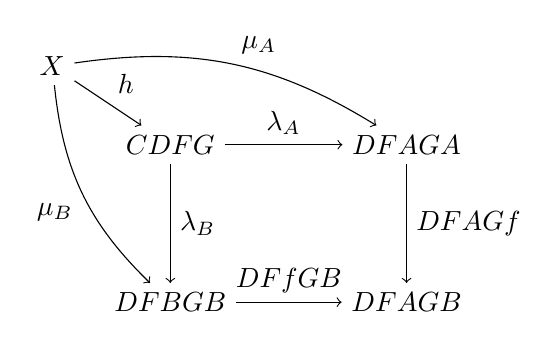
\begin{tikzpicture}[auto]
        \node (FG) at (0, 0) {$\arset{\funccat{C}{D}}{F}{G}$};
        \node (X) at (-1.5, 1) {$X$};
        \node (FAGA) at (3, 0) {$\arset{D}{FA}{GA}$};
        \node (FBGB) at (0, -2) {$\arset{D}{FB}{GB}$};
        \node (FAGB) at (3, -2) {$\arset{D}{FA}{GB}$};

        \draw[->] (FG) to node{$\lambda_A$}(FAGA);
        \draw[->] (X) to node{$h$}(FG);

        \draw[->] (FG) to node{$\lambda_B$}(FBGB);
        \draw[->,bend left = 20] (X) to node{$\mu_A$}(FAGA);
        \draw[->,bend right = 20] (X) to node[swap]{$\mu_B$}(FBGB);
        \draw[->] (FAGA) to node{$\arset{D}{FA}{Gf}$}(FAGB);
        \draw[->] (FBGB) to node{$\arset{D}{Ff}{GB}$}(FAGB);

      \end{tikzpicture}
    \end{center}
  \end{prop}
  \begin{proof}
    まず任意の対象$C$に対する$\cat{Set}$の射$\mor{\lambda_C}{\arset{\funccat{C}{D}}{F}{G}}{\arset{D}{FC}{GC}}$を定義する。\\
    任意の自然変換$\nat{\alpha}{F}{G}$に対して$\lambda_C(\alpha)=\alpha_C$とする。任意の自然変換はある対象に対する成分をただ一つ持つから、この操作は写像であり、$\cat{Set}$の射である。すると、
    \begin{align*}
      \arset{D}{FA}{Gf}\circ\lambda_A(\alpha)&=\arset{D}{FA}{Gf}(\alpha_A)&\text{($\lambda$の定義)}\\
      &=Gf\circ\alpha_A&\text{(射写像の定義)}\\
      \arset{D}{Ff}{GB}\circ\lambda_B(\alpha)&=\arset{D}{Ff}{GB}(\alpha_B)&\text{($\lambda$の定義)}\\
      &=\alpha_B\circ Ff&\text{(射写像の定義)}
    \end{align*}
  \end{proof}
  であり、$\alpha$の自然性から$Gf\circ\alpha_A=\alpha_B\circ Ff$が成り立つ。よって$\arset{D}{FA}{Gf}\circ\lambda_A=\arset{D}{Ff}{GB}\circ\lambda_B$を満たす。\\
  この等式では自然変換の成分が写像で与えられた場合の自然性を射写像を用いて課していることが分かる。\\
  次に射$h$の存在と一意性を示そうと思う。そこでまずは任意の対象$X$に終対象$1$を当てはめて考える。射$\mor{\mu_C}{1}{\arset{D}{FC}{GC}}$は射$\mor{\mu_A}{FA}{GA}$であり、任意の対象$C$に対して存在する。更に仮定より$\arset{D}{FA}{Gf}\circ\mu_A=\arset{D}{Ff}{GB}\circ\mu_B$が成り立つ。
  \begin{align*}
    \arset{D}{FA}{Gf}\circ\mu_A&=\arset{D}{Ff}{GB}\circ\mu_B\\
    \arset{D}{FA}{Gf}(\mu_A)&=\arset{D}{Ff}{GB}(\mu_B)&\text{(元と終対象からの射の同一視)}\\
    Gf\circ\mu_A&=\mu_B\circ Ff&\text{(射写像の定義)}
  \end{align*}
  よって自然変換の定義より、$\mu_C$は対象$C$成分であることが分かる。この自然変換を$\nat{\mu}{F}{G}$とすると、$\mu$は$\arset{\funccat{C}{D}}{F}{G}$の元である。すなわち$\mor{\mu}{1}{\arset{\funccat{C}{D}}{F}{G}}$と表せる。ここで$h=\mu$とすると$\lambda$は成分を取る写像であったから、$\mu_C=\lambda_C(\mu)=\lambda_C\circ\mu=\lambda_C\circ h$が成り立つ。
  \begin{center}
    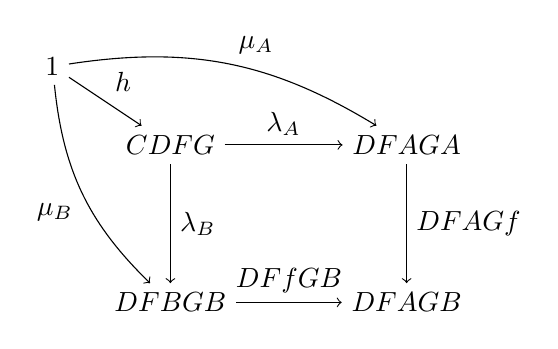
\begin{tikzpicture}[auto]
      \node (FG) at (0, 0) {$\arset{\funccat{C}{D}}{F}{G}$};
      \node (X) at (-1.5, 1) {$1$};
      \node (FAGA) at (3, 0) {$\arset{D}{FA}{GA}$};
      \node (FBGB) at (0, -2) {$\arset{D}{FB}{GB}$};
      \node (FAGB) at (3, -2) {$\arset{D}{FA}{GB}$};

      \draw[->] (FG) to node{$\lambda_A$}(FAGA);
      \draw[->] (X) to node{$h$}(FG);

      \draw[->] (FG) to node{$\lambda_B$}(FBGB);
      \draw[->,bend left = 20] (X) to node{$\mu_A$}(FAGA);
      \draw[->,bend right = 20] (X) to node[swap]{$\mu_B$}(FBGB);
      \draw[->] (FAGA) to node{$\arset{D}{FA}{Gf}$}(FAGB);
      \draw[->] (FBGB) to node{$\arset{D}{Ff}{GB}$}(FAGB);
    \end{tikzpicture}
  \end{center}
  一意性に関しても、$\mu_C=\lambda_C\circ h'$であるような$h'$が存在したとしても、$\mu_C={h'}_C$であり、自然変換の定義から$h'=\mu=h$が成り立つ。\\
  次に対象$1$を任意の対象$X$に拡張しよう。$X$の任意の元$x$に対し$\mu_C(x)$はある自然変換の$C$成分である。上記の議論から自然変換$h(x)_C=\mu_C(x)$であるため、自然変換$h(x)$は任意の$x$に対して一意に存在することになる。

  \begin{center}
    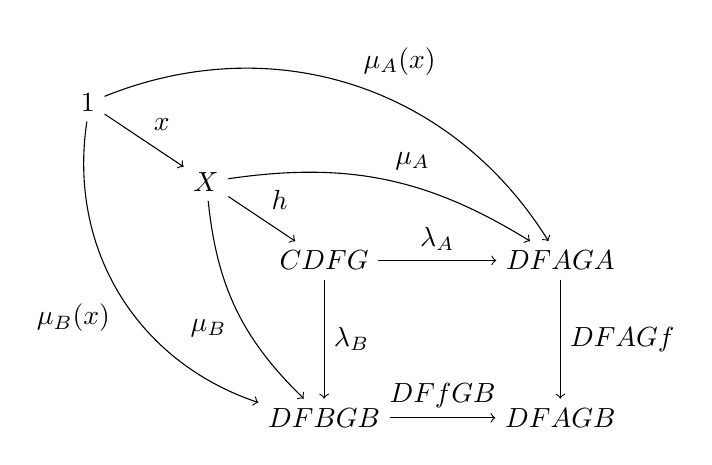
\begin{tikzpicture}[auto]
      \node (FG) at (0, 0) {$\arset{\funccat{C}{D}}{F}{G}$};
      \node (X) at (-1.5, 1) {$X$};
      \node (1) at (-3, 2) {$1$};
      \node (FAGA) at (3, 0) {$\arset{D}{FA}{GA}$};
      \node (FBGB) at (0, -2) {$\arset{D}{FB}{GB}$};
      \node (FAGB) at (3, -2) {$\arset{D}{FA}{GB}$};
      \draw[->] (FG) to node{$\lambda_A$}(FAGA);
      \draw[->] (X) to node{$h$}(FG);
      \draw[->] (1) to node{$x$}(X);
      \draw[->] (FG) to node{$\lambda_B$}(FBGB);
      \draw[->,bend left = 20] (X) to node{$\mu_A$}(FAGA);
      \draw[->,bend right = 20] (X) to node[swap]{$\mu_B$}(FBGB);
      \draw[->,bend left = 40] (1) to node{$\mu_A(x)$}(FAGA);
      \draw[->,bend right = 40] (1) to node[swap]{$\mu_B(x)$}(FBGB);
      \draw[->] (FAGA) to node{$\arset{D}{FA}{Gf}$}(FAGB);
      \draw[->] (FBGB) to node{$\arset{D}{Ff}{GB}$}(FAGB);
    \end{tikzpicture}
    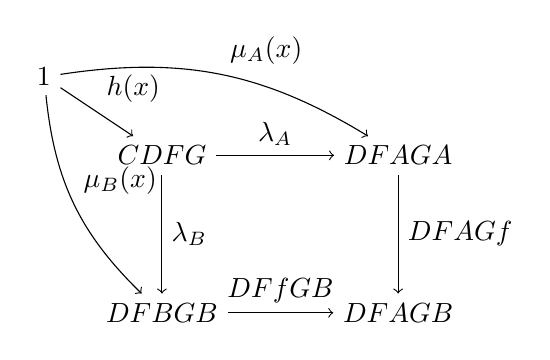
\begin{tikzpicture}[auto]
      \node (FG) at (0, 0) {$\arset{\funccat{C}{D}}{F}{G}$};
      \node (X) at (-1.5, 1) {$1$};
      \node (FAGA) at (3, 0) {$\arset{D}{FA}{GA}$};
      \node (FBGB) at (0, -2) {$\arset{D}{FB}{GB}$};
      \node (FAGB) at (3, -2) {$\arset{D}{FA}{GB}$};
      \draw[->] (FG) to node{$\lambda_A$}(FAGA);
      \draw[->] (X) to node{$h(x)$}(FG);
      \draw[->] (FG) to node{$\lambda_B$}(FBGB);
      \draw[->,bend left = 20] (X) to node{$\mu_A(x)$}(FAGA);
      \draw[->,bend right = 20] (X) to node{$\mu_B(x)$}(FBGB);
      \draw[->] (FAGA) to node{$\arset{D}{FA}{Gf}$}(FAGB);
      \draw[->] (FBGB) to node{$\arset{D}{Ff}{GB}$}(FAGB);
    \end{tikzpicture}
  \end{center}